% Written from cas-sc-template.tex of the Elsevier CAS bundle 2.4 (class cas-sc, single column).

% float (for the [H] figures and the [H] algorithm) is loaded before the class: the class loads hyperref,
% which adapts its float anchors only to a float package loaded before it (otherwise each figure anchor is
% written twice). \usepackage{float} in the package list below is then a no-op.
\RequirePackage{float}
\documentclass[a4paper,fleqn]{cas-sc}

\usepackage[numbers,sort&compress]{natbib}

% Packages the text needs beyond those the class loads.
\usepackage{float}            % H placement of figures and algorithms
\usepackage[most]{tcolorbox}
\usepackage{amsthm}
\usepackage{algorithm}
\usepackage{algpseudocode}    % part of the algorithmicx package

% Theorem-like environments, the "problem" box and numbering; independent of the document class.

% Numbering within sections
\numberwithin{equation}{section}

\theoremstyle{definition}
\newtheorem{definition}{Definition}[section]

\theoremstyle{plain}
\newtheorem{theorem}[definition]{Theorem}
\newtheorem{lemma}[definition]{Lemma}
\newtheorem{claim}[definition]{Claim}
\newtheorem{corollary}[definition]{Corollary}
\newtheorem{proposition}[definition]{Proposition}

\theoremstyle{remark}
\newtheorem{remark}[definition]{Remark}
\newtheorem{example}[definition]{Example}

% "problem" environment: framed statement of a computational problem
\newtcolorbox{problem}[1][]{%
  enhanced,
  colback=white,      % background color
  colframe=black,     % border color
  boxrule=0.8pt,      % border thickness
  arc=2pt,            % corner roundness
  left=6pt, right=6pt, top=6pt, bottom=6pt,
  title=\textbf{Problem: #1},
}

% Algorithm headers: every algorithm states its Input and Output;
% algpseudocode would print "Require:" and "Ensure:".
\algrenewcommand\algorithmicrequire{\textbf{Input:}}
\algrenewcommand\algorithmicensure{\textbf{Output:}}

% Notation macros; independent of the document class.

% Notation
\newcommand{\cp}{\operatorname{cp}}                  % value of a minimum cut-path
\newcommand{\diam}{\operatorname{diam}}
\newcommand{\tw}{\operatorname{tw}}
\newcommand{\torso}{\operatorname{torso}}
\newcommand{\OPT}{\mathrm{OPT}}
\newcommand{\ALG}{\mathrm{ALG}}
\newcommand{\MinCutPath}{\textsc{Min Cut-Path}}
\newcommand{\SSP}{\textsc{Separating Shortest Path}}
\newcommand{\ThreeSAT}{\textsc{3-SAT}}

% The class sets the text in STIX, which has no italic small caps: \textsc inside italic text takes the
% upright small caps that the font selection substitutes anyway; declared here so that it gives no warning.
\AtBeginDocument{%
  \DeclareFontShape{T1}{stix}{m}{scit}{<->ssub*stix/m/sc}{}%
  \DeclareFontShape{T1}{stix}{b}{scit}{<->ssub*stix/b/sc}{}}

% Key nologo of the class: the e-mail address is labelled "Email address:" instead of the icon
% thumbnails/cas-email.jpeg, so the manuscript also builds from one folder without sub-folders.
% Key H: the class's figure takes key-value options and would lose a plain [H] (it stores an empty placement);
% H is declared as a short form of the class's own key pos=H, so the figures keep the standard \begin{figure}[H].
\ExplSyntaxOn
\keys_set:nn { stm / mktitle } { nologo }
\keys_define:nn { cas / fig } { H .meta:n = { pos = H } }
\ExplSyntaxOff

\begin{document}
\let\WriteBookmarks\relax
\def\floatpagepagefraction{1}
\def\textpagefraction{.001}

\shorttitle{Min Cut-Path Problem}

\shortauthors{N. Micheľ}

\title[mode = title]{Min Cut-Path Problem}

\author[1]{Norbert Micheľ}

\cormark[1]

\ead{5344553@upjs.sk}

\affiliation[1]{organization={Institute of Computer Science, Faculty of Science, Pavol Jozef Šafárik University in Košice},
            addressline={Jesenná 5},
            postcode={040 01},
            postcodesep={},
            city={Košice},
            country={Slovakia}}

\cortext[1]{Corresponding author}

% The class writes the abstract body verbatim to a file and reads it back. The optional argument (the class's
% own heading) is given explicitly, so the class does not look ahead for one.
\begin{abstract}[\abstractname]
A cut-path between two vertices $u$ and $v$ of a graph is a set of edges that contains both a $u$--$v$ path and a cut separating $u$ from $v$.
In a network in which these edges are secured links, $u$ and $v$ communicate along the path, and every other route between them uses a secured link.
We study \MinCutPath{}, the problem of finding a cut-path with the fewest edges.
Let $c(u,v)$ be the size of a minimum cut separating $u$ from $v$, and let $d(u,v)$ be the distance between $u$ and $v$.
The union of a minimum cut and a shortest path is a cut-path with at most $c(u,v) + d(u,v) - 1$ edges, fewer than twice the minimum.
We prove that the decision version is NP-complete, already when the question is whether some shortest $u$--$v$ path is a cut separating $u$ from $v$.
Unless $\mathrm{P} = \mathrm{NP}$, the minimum cannot be approximated in polynomial time within a factor $1+\epsilon_0$, for some constant $\epsilon_0 > 0$, so the problem has no polynomial-time approximation scheme.
In contrast, the union is optimal in graphs of diameter two and in cactus graphs, where a minimum cut-path has exactly $c(u,v) + d(u,v) - 1$ edges.
In Erdős–Rényi random graphs on $n$ vertices with edge probability at least $\alpha \log n / n$ for a constant $\alpha > 1$, the union is within a factor $1+o(1)$ of the minimum with probability tending to one.
The decision version is fixed-parameter tractable with respect to the size of the cut-path.
\end{abstract}

\begin{keywords}
NP-completeness \sep edge connectivity \sep graph diameter \sep Erdős–Rényi graphs \sep average-case approximation
\end{keywords}

\maketitle

% PDF author field: \maketitle of the class fills it with the author list followed by ", ", which the
% PDF shows as a stray character; set after \maketitle, before the first page is written.
\hypersetup{pdfauthor={Norbert Micheľ}}

\section{Introduction}
\label{sec:introduction}

Let $u$ and $v$ be two distinct vertices of a graph.
A \emph{cut-path} between $u$ and $v$ is a set of edges that contains a $u$--$v$ path and a cut separating $u$ from $v$.
The \MinCutPath{} problem asks for a cut-path with the fewest edges, and $\cp(u,v)$ denotes their number.
In a communication network, the edges of a cut-path are the links that are secured against an adversary.
Then $u$ and $v$ communicate along the path, and every other route between them uses at least one secured link.

A shortest $u$--$v$ path and a minimum cut separating $u$ from $v$ are found in polynomial time, and every $u$--$v$ path shares an edge with every such cut.
Let $d(u,v)$ be the distance between $u$ and $v$, and let $c(u,v)$ be the size of a minimum cut separating them.
The union of a minimum cut and a shortest path is thus a cut-path with at most $c(u,v) + d(u,v) - 1$ edges, and every cut-path has at least $\max\{c(u,v), d(u,v)\}$ edges (Lemma~\ref{lem:basic-bounds}).
Hence the union has fewer than twice as many edges as a minimum cut-path (Corollary~\ref{cor:two-approximation}).
A minimum cut-path is in general not such a union.
A $u$--$v$ path $P$ and a cut $C$ form the cut-path $P \cup C$ with $|P| + |C| - |P \cap C|$ edges, so a longer path or a larger cut can give a smaller cut-path when the two share more edges.
The value $\cp(u,v)$ is the minimum, over all $u$--$v$ paths $P$, of $|P|$ plus the size of a minimum cut separating $u$ from $v$ in the graph without the edges of $P$ (Section~\ref{sec:fundamentals}).
A minimum cut-path may contain no minimum cut, or no shortest path, as the two graphs of Example~\ref{ex:strict} show.
We ask when the union of a minimum cut and a shortest path is optimal, and how hard \MinCutPath{} is when it is not.

\paragraph{Related work.}
Classical results relate a cut to a family of paths.
By Menger's theorem, $c(u,v)$ is the maximum number of pairwise edge-disjoint $u$--$v$ paths~\cite[Corollary~3.3.5]{Diestel2025}.
Results on minimum cuts alone include multi-terminal minimum cuts~\cite{GomoryHu1961}, cactus representations of all minimum cuts~\cite{NagamochiKameda1996} and the certification of 3-edge-connectivity~\cite{Mehlhorn2017Certifying}.
A cut-path consists of one path and one cut, and its size depends on the number of edges that the two share.

The problems closest to ours put a condition on a single $u$--$v$ path or on a single cut.
A $u$--$v$ path is \emph{non-disconnecting} if the removal of its edges leaves the graph connected.
Mao~\cite{Mao2021NonSeparating}, who calls such paths non-separating, proved that deciding whether a non-disconnecting $u$--$v$ path exists is NP-hard.
Abhinav et al.~\cite{Abhinav2022NonSeparating} proved that a shortest non-disconnecting $u$--$v$ path can be found in FPT time with respect to its length.
For the vertex version, in which the removal of the vertices of the path must leave the graph connected, they proved W[1]-hardness with respect to the length.
Such a path models a private channel whose removal keeps the rest of the network connected.
For two pairs of vertices, Eilam-Tzoreff~\cite{EilamTzoreff1998Disjoint} proved that it is NP-complete to decide whether some shortest path between the first pair is edge-disjoint from some path between the second pair, that is, whether its removal leaves the second pair connected.
We study the opposite requirement.
The \SSP{} problem asks whether the removal of the edges of some shortest $u$--$v$ path separates $u$ from $v$, or equivalently whether $\cp(u,v) = d(u,v)$.

Bazgan et al.~\cite{Bazgan2019MostVital} studied \textsc{Shortest Path Most Vital Edges}, the deletion of at most $k$ edges such that every remaining $u$--$v$ path has at least a given length.
For unit edge lengths, the deleted edges form a length-bounded edge cut, and the problem is NP-hard on graphs of diameter three and solvable in linear time on graphs of diameter at most two.
Baier et al.~\cite{Baier2010LengthBounded} proved that a minimum length-bounded edge cut is NP-hard to approximate within a factor of $1.1377$ when the paths to be destroyed are those with at most $L$ edges, for every fixed $L \geq 4$.
Such an edge set destroys all short $u$--$v$ paths, whereas a cut-path meets every $u$--$v$ path and contains one of them.

Other problems prescribe the structure of a cut.
\textsc{Network Diversion} asks for a minimal $u$--$v$ cut of at most $k+1$ edges that contains a prescribed edge.
Bentert et al.~\cite{Bentert2025NetworkDiversion} solved it in $O(n \log n)$ time on planar graphs with $n$ vertices and state that its complexity on general undirected graphs is open.
A \emph{matching cut} is the set of all edges between the two sides of a vertex partition, provided that this set is a matching.
Deciding whether a graph has a matching cut is solvable in polynomial time on graphs of diameter two and NP-complete on graphs of every fixed diameter at least three~\cite{LeLe2019MatchingCut}.
Komusiewicz et al.~\cite{Komusiewicz2020MatchingCut} gave kernels, single-exponential FPT algorithms and an exact exponential-time algorithm for this problem.
Marx, O'Sullivan and Razgon~\cite{Marx2013Separators} proved that all inclusion-minimal separators with at most $k$ vertices between two given vertices lie in a part of the graph whose torso has treewidth bounded by a function of $k$.
They derived FPT algorithms for separators with further properties, for example connected ones.

In these problems the condition concerns the cut alone.
In a cut-path, the cut and a path must together have few edges, and the edges of the path outside the cut may lie anywhere in the graph.
As with \textsc{Matching Cut} and with \textsc{Shortest Path Most Vital Edges} for unit edge lengths, graphs of diameter two form a polynomial case of \MinCutPath{} (Theorem~\ref{thm:diameter-two}).
To the best of our knowledge, neither \MinCutPath{} nor \SSP{} has been studied by other authors, under these or other names.

\paragraph{Our results.}
\begin{enumerate}
    \item \emph{Hardness.}
    \SSP{} is NP-complete (Theorem~\ref{thm:ssp-np-complete}), by a reduction from \ThreeSAT{} that produces graphs in which every vertex other than $u$ and $v$ has degree at most three.
    Hence the decision version of \MinCutPath{} is NP-complete (Theorem~\ref{thm:mcp-np-complete}), and so is deciding whether the lower bound $\cp(u,v) = d(u,v)$ is attained (Corollary~\ref{cor:lower-bound-attained}).
    The same reduction gives a constant $\epsilon_0 > 0$ such that, unless $\mathrm{P} = \mathrm{NP}$, no polynomial-time algorithm finds a cut-path with fewer than $(1+\epsilon_0)\cp(u,v)$ edges (Theorem~\ref{thm:no-ptas}).
    In particular, \MinCutPath{} has no polynomial-time approximation scheme.
    Unless $\mathrm{P} = \mathrm{NP}$, the best factor achievable in polynomial time therefore lies between $1+\epsilon_0$ and two.

    \item \emph{Two graph classes with an exact formula.}
    We prove that $\cp(u,v) = c(u,v) + d(u,v) - 1$ in graphs of diameter two (Theorem~\ref{thm:diameter-two}) and in cactus graphs (Theorem~\ref{thm:cut-two}).
    Cactus graphs are the connected graphs in which $c(x,y) \leq 2$ for every two distinct vertices $x$ and $y$ (Lemma~\ref{lem:cactus}, a folklore fact).
    In both classes the union of any minimum cut and any shortest path is therefore a minimum cut-path.
    In graphs of diameter two, $c(u,v) = \min\{\deg(u), \deg(v)\}$ by a theorem of Fricke, Oellermann and Swart (see~\cite[Theorem~11]{Stuart2009Eavesdropping}), so a minimum cut-path is found in linear time (Corollary~\ref{cor:diameter-two-degrees}).
    The hypotheses on all pairs of vertices cannot be replaced by $d(u,v) \leq 2$ or $c(u,v) \leq 2$ (Example~\ref{ex:strict}).

    \item \emph{Random graphs.}
    Erdős–Rényi random graphs with constant edge probability have diameter two with probability tending to one (Theorem~\ref{thm:random-diameter-two}), so the formula applies to them.
    For $n$ vertices and edge probability at least $\alpha \log n / n$ with a constant $\alpha > 1$, the union of a minimum cut and a shortest path has, with probability tending to one, at most $(1 + o(1))\cp(u,v)$ edges for all pairs $u, v$ at once (Theorem~\ref{thm:approximation-scheme}).
    The proof combines the bound $\cp(u,v) \geq c(u,v)$ with known bounds on the diameter~\cite{ChungLu2001} and on the edge connectivity~\cite{Bollobas2001} of these graphs.

    \item \emph{Parameterized complexity.}
    The decision version, which asks for a cut-path with at most $b$ edges, is fixed-parameter tractable with respect to $b$ (Theorem~\ref{thm:fpt}).
    It is decided in time $f(b)$ times a polynomial in the size of the graph.
    The proof gives no explicit bound on $f$.
\end{enumerate}

\paragraph{Techniques.}
The reduction from \ThreeSAT{} to \SSP{} builds a chain of cycles between $u$ and $v$.
Every shortest $u$--$v$ path of the chain uses one of the two halves of every cycle, and this choice encodes a truth value.
Further $u$--$v$ paths, the threads, cross the cycles, and a separating shortest path must share an edge with every thread.
Synchronization threads force the choices in all cycles of one variable to agree, and clause threads force the encoded truth assignment to satisfy every clause.
\SSP{} then reduces to \MinCutPath{}, because a cut-path with at most $d(u,v)$ edges is exactly a separating shortest path.
For the approximation hardness, we use that the threads are pairwise edge-disjoint, so a cut-path needs one further edge for every thread that its path misses.
Suppose that every truth assignment leaves a constant fraction of the clauses unsatisfied, which is NP-hard to distinguish from satisfiability when every variable occurs five times~\cite{Feige1998Threshold}.
Then every shortest $u$--$v$ path misses a constant fraction of the threads (Lemma~\ref{lem:unsatisfied-clauses}), and a longer path does not give a smaller cut-path (Lemma~\ref{lem:missed-threads}).

For Theorem~\ref{thm:fpt}, trying all cuts with at most $b$ edges takes time $|E|^{O(b)}$.
Instead, the treewidth reduction of Marx, O'Sullivan and Razgon~\cite{Marx2013Separators} places all inclusion-minimal cuts with at most $b$ edges in a part of the graph whose torso has treewidth bounded by a function of $b$.
The path of a cut-path may leave this part.
Marx, O'Sullivan and Razgon meet the same obstacle for connected separators and enlarge the part, whereas we add shortcuts whose lengths record the edges used outside.
The existence of a cut-path with at most $b$ edges is then expressed in monadic second-order logic and decided by Courcelle's theorem.

\paragraph{Organization.}
Section~\ref{sec:fundamentals} defines cut-paths and proves $\max\{c(u,v), d(u,v)\} \leq \cp(u,v) \leq c(u,v) + d(u,v) - 1$.
Sections~\ref{sec:np-completeness} and~\ref{sec:approximation} contain the hardness results, Sections~\ref{sec:diameter-two} and~\ref{sec:cut-two} the two graph classes, Section~\ref{sec:random-graphs} the random graphs, and Section~\ref{sec:fpt} the parameterized algorithm.
Section~\ref{sec:conclusion} lists open problems.

\section{Preliminaries}
\label{sec:fundamentals}

We use standard notation from graph theory and computational complexity and follow the conventions of~\cite{Diestel2025,Cormen2022}.
All graphs under consideration are finite, simple and undirected.

Most statements concern a graph $G = (V, E)$ and two distinct vertices $u, v \in V$.
The distance $d(u, v)$ is the length of a shortest $u$--$v$ path in $G$.
A set of edges whose removal disconnects $u$ from $v$ is a \emph{cut separating $u$ and $v$}, or a \emph{$u$--$v$ cut}.
The minimum size of a $u$--$v$ cut is denoted by $c(u, v)$ and called the \emph{cut-value} of $u$ and $v$.
We use the same notions and notation for any two distinct vertices $x, y$ of $G$, with $d(x, y) = \infty$ if $G$ contains no $x$--$y$ path.
For a vertex set $A$ with $u \in A$ and $v \notin A$, the set of all edges between $A$ and $V \setminus A$ is a $u$--$v$ cut, and every minimum $u$--$v$ cut is of this form (see the proof of Theorem~\ref{thm:diameter-two}).
All problems studied in this paper are defined with respect to these two distinguished vertices $u$ and $v$, and we assume that $u$ and $v$ lie in the same connected component of $G$.

We identify a path with its set of edges.
For a set of edges $F \subseteq E$, in particular for a path, we denote by $G \setminus F$ the graph obtained from $G$ by removing all edges of $F$.

\begin{definition}[Cut-Path]
\label{def:cut-path}
Let $G = (V, E)$ be a graph, and let $u, v \in V$ be two distinct vertices.
A \emph{cut-path} between $u$ and $v$ is a set of edges $S \subseteq E$ for which there exist subsets $P, C \subseteq S$ such that
    \begin{enumerate}
        \item $C$ is a cut separating $u$ and $v$ (i.e., removing $C$ disconnects $u$ from $v$), and
        \item $P$ is a path connecting $u$ and $v$.
    \end{enumerate}
\end{definition}

Every superset of a $u$--$v$ cut is a $u$--$v$ cut, so $S$ is a cut-path if and only if $S$ contains a $u$--$v$ path and $G \setminus S$ contains no $u$--$v$ path.
Figure~\ref{fig:cut-path} shows a cut-path schematically.

\begin{figure}[H]
    \centering
    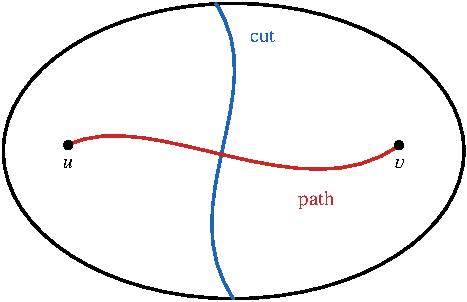
\includegraphics{cut-path.pdf}
    \caption{A cut-path between $u$ and $v$ (schematic)}
    \label{fig:cut-path}
\end{figure}

\begin{definition}[Value of Minimum Cut-Path]
\label{def:cp-value}
Let $G = (V, E)$ be a graph, and let $u, v \in V$ be two distinct vertices.
The minimum size of a cut-path between $u$ and $v$ is denoted by $\cp(u, v)$:
\[
\cp(u, v) = \min\{ |S| \mid S \text{ is a cut-path between } u \text{ and } v \}.
\]
\end{definition}

Since $u$ and $v$ lie in the same connected component, the edge set $E$ contains a $u$--$v$ path, and removing all edges of $E$ disconnects $u$ from $v$ because $u \neq v$.
Hence $E$ is a cut-path, and the minimum in Definition~\ref{def:cp-value} exists.
A cut-path $S$ with $|S| = \cp(u, v)$ is called a \emph{minimum cut-path} between $u$ and $v$.
For a fixed $u$--$v$ path $P$, a set $S \supseteq P$ is a cut-path if and only if $S \setminus P$ is a $u$--$v$ cut of $G \setminus P$.
Hence $\cp(u, v)$ is the minimum, over all $u$--$v$ paths $P$, of $|P|$ plus the cut-value of $u$ and $v$ in $G \setminus P$.

\begin{problem}[\MinCutPath{} (Optimization Version)]
Let $G=(V,E)$ be an undirected graph and $u,v \in V$ distinct vertices.
Cut-paths are defined in Definition~\ref{def:cut-path}.
The optimization version of the \MinCutPath{} problem is defined as follows:

\begin{center}
\begin{tabular}{p{0.18\linewidth}p{0.75\linewidth}}
\textbf{Input:} & A graph $G=(V,E)$ and vertices $u,v \in V$. \\
\textbf{Output:} & A minimum cut-path between $u$ and $v$ and its size $\cp(u,v)$.
\end{tabular}
\end{center}
\end{problem}

\begin{lemma}[Basic Bounds]
\label{lem:basic-bounds}
Let $G = (V, E)$ be a graph, and let $u, v \in V$ be two distinct vertices. Then
\[
\max\{c(u, v), d(u, v)\} \leq \cp(u, v) \leq c(u, v) + d(u, v) - 1.
\]
In particular, if $c(u, v) = 1$ or $d(u, v) = 1$, then $\cp(u, v) = c(u, v) + d(u, v) - 1$.
\end{lemma}

\begin{proof}
The lower bound holds because every cut-path contains a $u$--$v$ cut, which has at least $c(u, v)$ edges, and a $u$--$v$ path, which has at least $d(u, v)$ edges.
For the upper bound, let $C$ be a minimum $u$--$v$ cut and let $P$ be a shortest $u$--$v$ path.
The set $C \cup P$ is a cut-path by Definition~\ref{def:cut-path}, since it contains the cut $C$ and the path $P$.
Since removing $C$ disconnects $u$ from $v$, the path $P$ contains at least one edge of $C$.
Hence $|C \cup P| \leq |C| + |P| - 1 = c(u, v) + d(u, v) - 1$.
If $c(u, v) = 1$, the lower bound gives $\cp(u, v) \geq d(u, v) = c(u, v) + d(u, v) - 1$.
If $d(u, v) = 1$, it gives $\cp(u, v) \geq c(u, v) = c(u, v) + d(u, v) - 1$.
In both cases the lower and the upper bound coincide.
\end{proof}

\begin{corollary}
\label{cor:two-approximation}
Let $G = (V, E)$ be a graph, let $u, v \in V$ be two distinct vertices, let $C$ be a minimum $u$--$v$ cut, and let $P$ be a shortest $u$--$v$ path.
Then $|C \cup P| \leq 2\cp(u, v) - 1$.
\end{corollary}

\begin{proof}
By the proof of Lemma~\ref{lem:basic-bounds} and by its lower bound,
\[
|C \cup P| \leq c(u, v) + d(u, v) - 1 \leq 2\max\{c(u, v), d(u, v)\} - 1 \leq 2\cp(u, v) - 1. \qedhere
\]
\end{proof}

Hence the union of a minimum cut and a shortest path approximates a minimum cut-path within a factor of two.

For random graphs (Section~\ref{sec:random-graphs}), we use the following notion of approximation.
Let $\mathcal{I}(n)$ denote the set of all input instances of size $n$.
For an instance $X \in \mathcal{I}(n)$, let $\OPT(X)$ denote the optimal value of the objective function, that is, the minimum for a minimization problem and the maximum for a maximization problem.

\begin{definition}[Average $(1+\epsilon)$-Approximation Scheme]
\label{def:approximation-scheme}
Let $\epsilon > 0$. An algorithm $\ALG$ is called an \emph{average $(1+\epsilon)$-approximation scheme} if the following three conditions hold.
\begin{enumerate}
    \item $\ALG$ is a polynomial-time algorithm, i.e., its running time is bounded by a polynomial in $n$.
    \item For each input size $n$, there exists a subset of inputs $\mathcal{I}_{\ALG}^{\mathrm{opt}}(n) \subseteq \mathcal{I}(n)$ such that for every input $X \in \mathcal{I}_{\ALG}^{\mathrm{opt}}(n)$, the value $\ALG(X)$ of the solution computed by $\ALG$ satisfies
    \[
    \frac{\ALG(X)}{\OPT(X)} < 1+\epsilon \quad \text{(for minimization problems)}
    \]
    \[
    \frac{\OPT(X)}{\ALG(X)} < 1+\epsilon \quad \text{(for maximization problems)},
    \]
    \item In addition, the algorithm is average-case in the sense that, for a given probability distribution on $\mathcal{I}(n)$, a random input $X$ of size $n$ satisfies
    \[
    \lim_{n \to \infty} \mathbb{P}\bigl(X \in \mathcal{I}_{\ALG}^{\mathrm{opt}}(n)\bigr) = 1.
    \]
\end{enumerate}
\end{definition}

\section{NP-completeness of the Min Cut-Path Problem}
\label{sec:np-completeness}
We prove that the decision version of the \MinCutPath{} problem is NP-complete by a reduction from the \ThreeSAT{} problem.

\begin{problem}[\ThreeSAT]
Let $U = \{x_1, x_2, \dots, x_n\}$ be a finite set of Boolean variables, and let
$\mathcal{C} = \{C_1, C_2, \dots, C_m\}$ be a collection of clauses, where each clause
$C_k$ is a disjunction of exactly three literals, not necessarily distinct, and each literal is either a variable $x_i$ or its negation $\neg x_i$.

The \ThreeSAT{} decision problem is defined as follows:

\begin{center}
\begin{tabular}{p{0.12\linewidth}p{0.8\linewidth}}
\textbf{Input:} & A finite set of Boolean variables $U$ and a collection $\mathcal{C}$ of clauses, each containing exactly three literals.\\
\textbf{Question:} & Does there exist a truth assignment $\tau: U \rightarrow \{\mathsf{true}, \mathsf{false}\}$ such that every clause $C_k \in \mathcal{C}$ evaluates to \textsf{true} under $\tau$?
\end{tabular}
\end{center}
\end{problem}

\ThreeSAT{} is NP-complete~\cite{Cook1971Complexity,Karp1972Reducibility}.
These papers allow clauses with fewer than three literals, and such a clause is padded by repeating one of its literals.
Throughout this section, $n$ and $m$ denote the numbers of variables and clauses of the \ThreeSAT{} instance under consideration.

The proof has two steps and uses an intermediate problem, \SSP.
First, we show that \SSP{} is NP-complete by a polynomial-time reduction from \ThreeSAT{} (Section~\ref{sec:ssp}).
Second, we reduce \SSP{} to \MinCutPath{} (Section~\ref{sec:ssp-to-mcp}).

\subsection{The Separating Shortest Path Problem}\label{sec:ssp}

\begin{problem}[\SSP]
Let $G = (V,E)$ be an undirected graph and let $u,v \in V$ be two distinct vertices.
A shortest $u$--$v$ path $P$ is called a \emph{separating shortest path} if the graph $G \setminus P$ contains no $u$--$v$ path.
The \SSP{} decision problem is defined as follows:

\begin{center}
\begin{tabular}{p{0.12\linewidth}p{0.8\linewidth}}
\textbf{Input:} & A graph $G = (V,E)$ and two distinct vertices $u,v \in V$.\\
\textbf{Question:} & Does there exist a shortest $u$--$v$ path in $G$ that is a separating shortest path?
\end{tabular}
\end{center}
\end{problem}

Unlike \MinCutPath, \SSP{} is not an optimization problem.
A solution is a single separating shortest $u$--$v$ path, which is a cut-path of size $d(u,v)$ (see the proof of Theorem~\ref{thm:mcp-np-complete}).

\subsubsection{Gadgets and Basic Operations for the Reduction}

The reduction from \ThreeSAT{} to \SSP{} is built from \emph{gadgets} and \emph{basic operations} on them.
The construction consists of two parts:
\begin{enumerate}
    \item the \emph{base structure}, also referred to as the \emph{chain};
    \item the \emph{threads}, which are threaded through the chain.
\end{enumerate}
Figure~\ref{fig:chain-threads} shows both parts.

\begin{figure}[H]
    \centering
    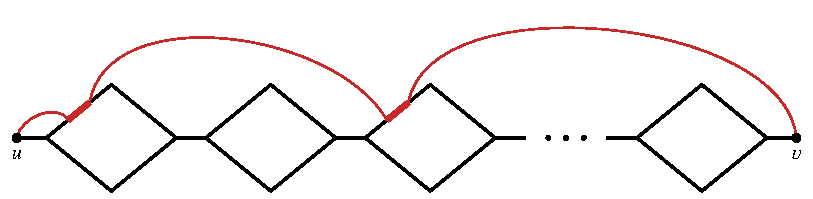
\includegraphics{chain-threads.pdf}
    \caption{Layout of the construction: the chain (black) and a thread (red)}
    \label{fig:chain-threads}
\end{figure}

\paragraph{Chain.}
\begin{definition}[Chain Link]
\label{def:chain-link}
Let $G=(V,E)$ be a graph and let $p,q \in V$ be two distinct vertices.
A \emph{$(p,q)$-chain link} is a subgraph $L \subseteq G$ such that:
\begin{enumerate}
    \item $L$ is a cycle in $G$ through $p$ and $q$;
    \item the two $p$--$q$ paths of $L$ have equal length.
\end{enumerate}
We refer to one of the two $p$--$q$ paths as the \emph{positive path} of the chain link and to the other as the \emph{negative path}.
\end{definition}

Figure~\ref{fig:chain-link} shows a chain link.

\begin{figure}[H]
    \centering
    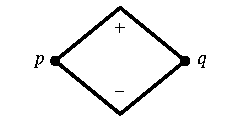
\includegraphics{chain-link.pdf}
    \caption{A chain link}
    \label{fig:chain-link}
\end{figure}

\begin{definition}[Chain]
\label{def:chain}
Let $G=(V,E)$ be a graph, and let $u,v\in V$.
We say that $G$ is a \emph{$u$--$v$ chain} with $r$ chain links if it is the union of edge-disjoint subgraphs
\[
G = H_1 \cup L_1 \cup H_2 \cup L_2 \cup \cdots \cup L_r \cup H_{r+1},
\]
where:
\begin{enumerate}
    \item each $H_i$ consists of a single edge with end-vertices $p_i,q_i$;
    \item each $L_i$ is a $(q_i,p_{i+1})$-chain link;
    \item the first end-vertex $p_1$ coincides with $u$ and the last end-vertex $q_{r+1}$ coincides with $v$;
    \item two of these subgraphs share a vertex only if they are consecutive, and then they share exactly one vertex ($q_i$ or $p_{i+1}$).
\end{enumerate}
\end{definition}

Every $u$--$v$ path in a chain traverses all single edges and, in each chain link, either its positive or its negative path (Figure~\ref{fig:chain}).

\begin{figure}[H]
    \centering
    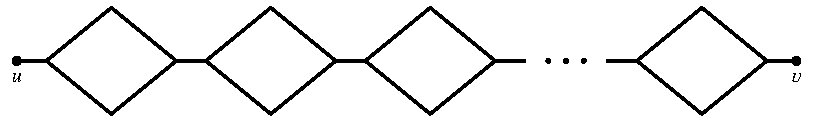
\includegraphics{chain.pdf}
    \caption{A chain}
    \label{fig:chain}
\end{figure}

In the reduction, every chain link has one of three types:
\begin{enumerate}
    \item \textbf{Initialization chain link.}
    For each variable $x_i$ we introduce an initialization chain link, denoted $I_i$.
    This link marks the beginning of the part of the chain that corresponds to the variable $x_i$.

    \item \textbf{Terminal chain link.}
    For each variable $x_i$ we also introduce a terminal chain link, denoted $T_i$.
    This link marks the end of the part of the chain associated with the variable $x_i$.

    \item \textbf{Literal chain link.}
    For each clause $C_k = (\ell_1 \vee \ell_2 \vee \ell_3)$ and each $j \in \{1,2,3\}$, let $x_i$ be the variable of the literal $\ell_j$.
    We introduce a literal chain link, denoted $L_{j,k}$.
    This link represents the occurrence of the variable $x_i$ as the $j$-th literal of the clause $C_k$.
\end{enumerate}
Hence the construction contains $n$ initialization, $n$ terminal and $3m$ literal chain links, $2n + 3m$ in total.
The chain links that belong to one variable are consecutive in the chain, as illustrated in Figure~\ref{fig:chain-link-types}.

\begin{figure}[H]
    \centering
    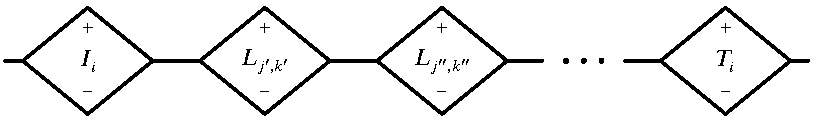
\includegraphics{chain-link-types.pdf}
    \caption{Chain links of a variable $x_i$: the initialization link, the literal links, and the terminal link}
    \label{fig:chain-link-types}
\end{figure}

\paragraph{Threads and threading.}
\begin{definition}[Thread]
\label{def:thread}
Let $G=(V,E)$ be a graph containing a $u$--$v$ chain with chain links $L_1,L_2,\dots,L_r$.
A \emph{thread} is a $u$--$v$ path $P$ in $G$ such that:
\begin{enumerate}
    \item for each chain link $L_i$, the path $P$ shares at most one edge with $L_i$;
    \item $P$ contains none of the single edges of the chain.
\end{enumerate}
\end{definition}

The threads of the construction are created by the procedure $\textsc{Thread}$ (Section~\ref{sec:reduction-construction}).
From now on, the word thread refers to these paths only.
Any two of them are edge-disjoint and share only the vertices $u$ and $v$.

\begin{definition}[Threading]
\label{def:threading}
Let $L$ be a chain link in a $u$--$v$ chain, and let $P$ be a thread under construction that does not yet pass through $L$.
The \emph{threading operation} on $(P,L)$ consists of the following elementary steps:
\begin{enumerate}
    \item Select an edge $e=\{x,y\}$ of $L$ that is not used by any existing thread.
    \item Subdivide $e$ into a path $x$--$z_1$--$z_2$--$y$ of three edges, introducing two new vertices $z_1,z_2$.
    \item Extend $P$ so that it traverses the middle edge $\{z_1,z_2\}$, called the \emph{crossing edge}, as its unique crossing of the chain link $L$.
\end{enumerate}
If the selected edge $e$ belongs to the positive path of $L$, we say that $P$ is \emph{positively threaded through $L$}.
If $e$ belongs to the negative path of $L$, we say that $P$ is \emph{negatively threaded through $L$}.
In general, we say that the thread $P$ is \emph{threaded through $L$ at the edge $e$}.
\end{definition}

Figure~\ref{fig:threading} shows the threading operation.

\begin{figure}[H]
    \centering
    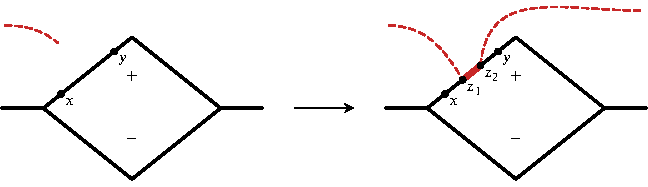
\includegraphics{threading.pdf}
    \caption{The threading operation}
    \label{fig:threading}
\end{figure}

Every thread has one of three types:
\begin{enumerate}
    \item \textbf{2-synchronization thread.}
    This thread passes through an initialization chain link $I_i$ and the corresponding terminal chain link $T_i$ (Figure~\ref{fig:two-synchronization}).
    Threads of this type force every separating shortest path to traverse paths of the same sign in $I_i$ and $T_i$ (Lemmas~\ref{lem:chain-paths} and~\ref{lem:synchronization}).

    \item \textbf{3-synchronization thread.}
    This thread passes through the initialization chain link $I_i$, a literal chain link $L_{j,k}$ of an occurrence of $x_i$, and the terminal chain link $T_i$ corresponding to the same variable $x_i$ (Figure~\ref{fig:three-synchronization}).
    Threads of this type force every separating shortest path to traverse the path of this sign in $L_{j,k}$ as well (Lemma~\ref{lem:synchronization}).

    \item \textbf{Clause thread.}
    For each clause $C_k = (\ell_{1} \vee \ell_{2} \vee \ell_{3})$, a clause thread is introduced that passes through the three literal chain links $L_{1,k}$, $L_{2,k}$, $L_{3,k}$ corresponding to $\ell_{1}, \ell_{2}, \ell_{3}$ (Figure~\ref{fig:clause-thread}).
    It encodes the clause in the sense that a separating shortest path exists only if at least one of the three literals is satisfied (Lemma~\ref{lem:clause-threads}).
\end{enumerate}

\begin{figure}[H]
    \centering
    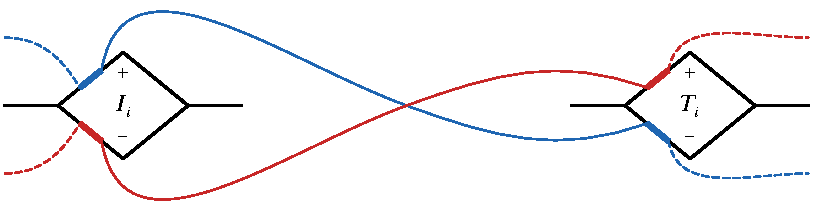
\includegraphics{two-synchronization-threads.pdf}
    \caption{The two 2-synchronization threads of a variable $x_i$}
    \label{fig:two-synchronization}
\end{figure}

\begin{figure}[H]
    \centering
    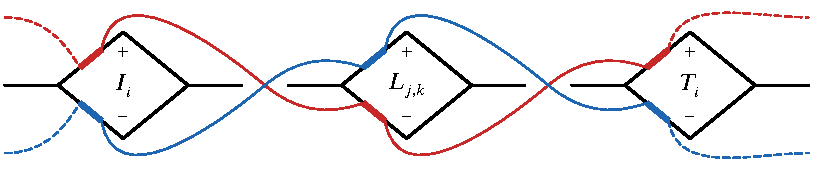
\includegraphics{three-synchronization-threads.pdf}
    \caption{The two 3-synchronization threads of a literal chain link $L_{j,k}$}
    \label{fig:three-synchronization}
\end{figure}

\begin{figure}[H]
    \centering
    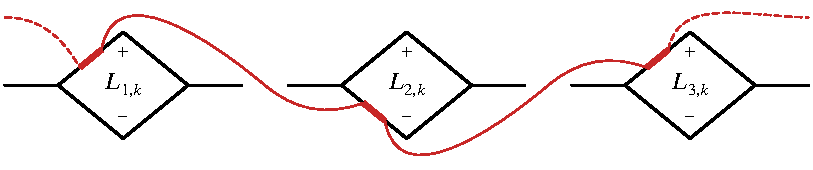
\includegraphics{clause-thread.pdf}
    \caption{The clause thread of a clause $C_k = (x_1 \vee \neg x_2 \vee x_3)$}
    \label{fig:clause-thread}
\end{figure}

\subsubsection{The Construction}
\label{sec:reduction-construction}
Given an instance of \ThreeSAT, we construct a graph $G$ with two distinguished vertices $u,v$ such that $G$ contains a separating shortest $u$--$v$ path if and only if the given formula is satisfiable.

\paragraph{Auxiliary procedures.}
The reduction uses the following auxiliary procedures:
\begin{itemize}
    \item $\textsc{BuildChain}(u,v,r)$: constructs a $u$--$v$ chain with $r$ chain links, where each chain link is realized as a $4$-cycle.
    \item $\textsc{Thread}(u,v,[(K_1,\sigma_1),\dots,(K_t,\sigma_t)])$: creates a new thread from $u$ to $v$ that passes through the chain links $K_1,\dots,K_t$ in this order, where $\sigma_h \in \{+,-\}$ specifies whether the thread is threaded through $K_h$ positively or negatively.
    The $t$ crossing edges are joined to each other and to the vertices $u$ and $v$ by $t+1$ new, internally vertex-disjoint paths of one edge each, which we call the \emph{connecting paths} of the thread.
    The procedure $\textsc{Calibrate}$ subdivides them later.
    \item $\textsc{Calibrate}(G)$: equalizes the lengths of the relevant paths in two steps.
    First, in every chain link whose positive and negative paths have different lengths, an edge of the shorter path that is not a crossing edge is subdivided repeatedly until both paths have the same length.
    Second, every connecting path of every thread is subdivided until it has exactly $\Lambda$ edges, where $\Lambda$ denotes the number of edges of a $u$--$v$ path in the resulting chain.
\end{itemize}

\paragraph{Auxiliary notation.}
We use the following notation:
\begin{itemize}
    \item Literals: every literal $\ell$ of the formula is identified with its position, $\ell[0] = j$ and $\ell[1] = k$ if $\ell$ is the $j$-th literal of the clause $C_k$.
    Its literal chain link is $L_{\ell[0],\ell[1]}$.
    \item Literals of a variable: $\mathcal{M}$ maps every variable $x_i$ to the list $\mathcal{M}[x_i]$ of all literals of the formula whose variable is $x_i$, that is, of all occurrences of $x_i$ and $\neg x_i$.
    \item Sign function: for each literal $\ell$ we define
\[
s(\ell) =
\begin{cases}
+ & \text{if $\ell = x_i$ for some variable $x_i$,}\\
- & \text{if $\ell = \neg x_i$ for some variable $x_i$.}
\end{cases}
\]
\end{itemize}

\paragraph{The graph of the reduction.}
Algorithm~\ref{alg:reduction} constructs the graph $G$ and the vertices $u,v$.
From now on, $G$, $u$ and $v$ denote its output.

\begin{algorithm}[H]
\caption{Reduction from \ThreeSAT{} to \SSP}
\label{alg:reduction}
\begin{algorithmic}[1]
\Require Variables $U=\{x_1,\dots,x_n\}$, clauses $\mathcal{C}=\{C_1,\dots,C_m\}$
\Ensure Graph $G$, vertices $u,v$
\State $n \gets |U|$, $m \gets |\mathcal{C}|$
\State $G \gets \textsc{BuildChain}(u,v,2n+3m)$
\State $\mathcal{M} \gets$ map from each variable to the list of its literals
\For{$i \gets 1$ to $n$}
    \State $\mathit{Lits} \gets \mathcal{M}[x_i]$
    \State reserve the next $2+|\mathit{Lits}|$ free chain links
    \State label the first of them as $I_i$ and the last as $T_i$
    \For{each $\ell \in \mathit{Lits}$}
        \State label the next free reserved link as $L_{\ell[0],\ell[1]}$
    \EndFor
\EndFor
\For{$i \gets 1$ to $n$}
    \State $\textsc{Thread}(u,v,[(I_i,+),(T_i,-)])$
    \State $\textsc{Thread}(u,v,[(I_i,-),(T_i,+)])$
    \State $\mathit{Lits} \gets \mathcal{M}[x_i]$
    \For{each $\ell \in \mathit{Lits}$}
        \State $\textsc{Thread}(u,v,[(I_i,+),(L_{\ell[0],\ell[1]},-),(T_i,+)])$
        \State $\textsc{Thread}(u,v,[(I_i,-),(L_{\ell[0],\ell[1]},+),(T_i,-)])$
    \EndFor
\EndFor
\For{$k \gets 1$ to $m$}
    \State $\ell_1,\ell_2,\ell_3 \gets$ the literals of $C_k$
    \State $\textsc{Thread}(u,v,[(L_{\ell_1[0],\ell_1[1]},s(\ell_1)),(L_{\ell_2[0],\ell_2[1]},s(\ell_2)),(L_{\ell_3[0],\ell_3[1]},s(\ell_3))])$
\EndFor
\State $\textsc{Calibrate}(G)$
\State \Return $G$, $u$, $v$
\end{algorithmic}
\end{algorithm}

Informally, the chain consists of $n$ consecutive blocks, one for each variable.
The block of $x_i$ starts with $I_i$, ends with $T_i$, and contains the literal chain links of all occurrences of $x_i$ in between.
Each variable receives a pair of 2-synchronization threads, each occurrence of a variable receives a pair of 3-synchronization threads, and each clause receives one clause thread.
Every thread passes through at least two chain links, so it has at least two crossing edges.
After the calibration, the subdivided $4$-cycles are again chain links, and the chain in $G$ is a $u$--$v$ chain in the sense of Definition~\ref{def:chain}.
Every $u$--$v$ path of this chain has exactly $\Lambda$ edges, and so has every connecting path.

The construction is well defined.
At the beginning, each of the two paths of a chain link has two edges.
A threading replaces an edge that no thread uses by two such edges and a crossing edge, so it always finds an edge on the requested path.
Between its first threading and the calibration, the two paths of a chain link may differ in length, and we still call the cycle a chain link.
The end-vertices of a crossing edge are new vertices, so distinct crossing edges share no vertex, and each of these end-vertices is incident to two edges of its chain link and to exactly one connecting path.
A thread visits its chain links in the order of its list, which for a clause thread need not be their order along the chain.
The statements below hold for every choice of the edges that the threadings and $\textsc{Calibrate}$ subdivide.

\subsubsection{Correctness of the Reduction}
\label{sec:reduction-correctness}
\begin{definition}[Chain Path, Hitting, Consistency]
\label{def:chain-path}
A \emph{chain path} is a $u$--$v$ path of the chain in $G$.
A chain path $P$ \emph{hits} a thread if $P$ and the thread share an edge.
A chain path is \emph{consistent} if, for every variable $x_i$, it traverses paths of the same sign in all chain links of the block of $x_i$.
\end{definition}

A chain path is determined by choosing, in every chain link, either its positive or its negative path, and a thread shares only its crossing edges with the chain.
Hence a chain path $P$ hits a thread created by $\textsc{Thread}(u,v,\allowbreak[(K_1,\sigma_1),\dots,(K_t,\sigma_t)])$ if and only if, for some $h$, the path $P$ traverses the path of $K_h$ with the sign $\sigma_h$.

Every thread is a $u$--$v$ path in $G$.
Therefore, a chain path $P$ can be separating only if it hits every thread.

Consistent chain paths correspond to truth assignments.
For such a path, we set $\tau(x_i)=\mathsf{true}$ if the path traverses the positive paths in the block of $x_i$, and $\tau(x_i)=\mathsf{false}$ otherwise.
Conversely, every truth assignment $\tau$ determines a consistent chain path, which traverses, in all chain links of the block of $x_i$, the positive path if $\tau(x_i)=\mathsf{true}$ and the negative path if $\tau(x_i)=\mathsf{false}$.
We call it the \emph{consistent chain path of~$\tau$}.

\begin{lemma}[Shortest Paths]
\label{lem:chain-paths}
All chain paths have $\Lambda$ edges, and every other $u$--$v$ path in $G$ has more than $\Lambda$ edges.
In particular, the shortest $u$--$v$ paths in $G$ are exactly the chain paths.
\end{lemma}

\begin{proof}
After the calibration, all chain paths have the same length $\Lambda$.
Let $Q$ be a $u$--$v$ path in $G$ that is not a chain path.
We show that $Q$ contains a whole connecting path and at least one further edge.
By Definition~\ref{def:chain}, every $u$--$v$ path that uses only edges of the chain is a chain path, and the edges of $G$ outside the chain are the edges of the connecting paths.
Hence $Q$ contains an edge of some connecting path.

The internal vertices of a connecting path have degree two in $G$, because the procedure $\textsc{Thread}$ creates the connecting paths as new, internally vertex-disjoint paths and $\textsc{Calibrate}$ subdivides them only by new vertices of degree two.
Since $u$ and $v$ are not internal vertices of a connecting path, $Q$ contains the whole connecting path, which has $\Lambda$ edges.
Every thread has at least two crossing edges, so every connecting path has an end-vertex on a crossing edge, and no connecting path joins $u$ and $v$ directly.
Hence $Q$ contains at least one further edge, and $|Q| > \Lambda$.
\end{proof}

\begin{lemma}[Synchronization]
\label{lem:synchronization}
A chain path hits all synchronization threads if and only if it is consistent.
\end{lemma}

\begin{proof}
Let $P$ be a chain path and let $x_i$ be a variable.
By Algorithm~\ref{alg:reduction}, the block of $x_i$ consists of $I_i$, the literal chain links $L_{\ell[0],\ell[1]}$ with $\ell \in \mathcal{M}[x_i]$, and $T_i$.
\begin{itemize}
    \item \emph{2-synchronization threads.} The chain path $P$ hits both 2-synchronization threads of the variable $x_i$ (Figure~\ref{fig:two-synchronization}) if and only if it traverses paths of the same sign in $I_i$ and in $T_i$.
    Indeed, the thread $[(I_i,+),(T_i,-)]$ is hit exactly when $P$ traverses the positive path in $I_i$ or the negative path in $T_i$, and the thread $[(I_i,-),(T_i,+)]$ exactly when $P$ traverses the negative path in $I_i$ or the positive path in $T_i$.
    \item \emph{3-synchronization threads.} If $P$ traverses paths of the same sign in $I_i$ and $T_i$, then it hits both 3-synchronization threads of a literal chain link $L_{j,k}$ of this block (Figure~\ref{fig:three-synchronization}) if and only if it traverses the path of this sign in $L_{j,k}$ as well.
    Indeed, the thread $[(I_i,+),(L_{j,k},-),(T_i,+)]$ is hit exactly when $P$ uses the positive path in $I_i$ or $T_i$ or the negative path in $L_{j,k}$.
    The thread $[(I_i,-),(L_{j,k},+),(T_i,-)]$ is hit exactly when $P$ uses the negative path in $I_i$ or $T_i$ or the positive path in $L_{j,k}$.
\end{itemize}
Suppose that $P$ hits all synchronization threads.
By the first item, $P$ traverses paths of the same sign in $I_i$ and $T_i$, and by the second item, it traverses the path of this sign in every literal chain link of the block as well.
Conversely, if $P$ traverses paths of the same sign in all chain links of the block of $x_i$, then both items show that $P$ hits all synchronization threads of $x_i$.
Since this holds for every variable $x_i$, a chain path hits all synchronization threads if and only if it traverses paths of the same sign in all chain links of every block, that is, if and only if it is consistent.
\end{proof}

\begin{lemma}[Clause Threads]
\label{lem:clause-threads}
Let $P$ be a consistent chain path and let $\tau$ be its truth assignment.
Then $P$ hits all clause threads if and only if $\tau$ satisfies every clause.
\end{lemma}

\begin{proof}
Let $C_k = (\ell_1 \vee \ell_2 \vee \ell_3)$ be a clause.
The path $P$ hits the clause thread of $C_k$ if and only if, for some $j$, it traverses the path of $L_{j,k}$ with the sign $s(\ell_j)$, i.e., if and only if $\tau$ satisfies the literal $\ell_j$.
Indeed, if $x_i$ is the variable of $\ell_j$, then $P$ traverses the positive path of $L_{j,k}$ exactly when $\tau(x_i)=\mathsf{true}$, and $s(\ell_j) = +$ exactly when $\ell_j = x_i$.
Thus a consistent chain path hits all clause threads if and only if its truth assignment satisfies every clause.
\end{proof}

\begin{lemma}[Separation]
\label{lem:separating}
Let $\tau$ be a truth assignment that satisfies every clause, and let $P$ be the consistent chain path of $\tau$.
Then $P$ is a separating shortest $u$--$v$ path in $G$.
\end{lemma}

\begin{proof}
By Lemma~\ref{lem:chain-paths}, $P$ is a shortest $u$--$v$ path.
It remains to show that $G \setminus P$ contains no $u$--$v$ path.
We first describe the graph $G \setminus P$ and then follow a $u$--$v$ path of $G \setminus P$ in a graph that records which paths of the chain links the connecting paths join.

\paragraph{The graph $G \setminus P$.}
All single edges of the chain lie on $P$.
In every chain link, only the path not traversed by $P$ remains in $G \setminus P$, and we call it the \emph{unused path} of the chain link.
Unused paths of distinct chain links are vertex-disjoint and contain neither $u$ nor $v$.
Every edge of $G \setminus P$ lies on an unused path or on a connecting path.
An end of a connecting path is $u$, $v$, or an end-vertex of a crossing edge, and such an end-vertex is an internal vertex of exactly one of the two paths of its chain link.
If $P$ traverses this path, the end-vertex has degree one in $G \setminus P$, because two of its three edges lie on $P$.

\paragraph{The transition graph.}
For a chain link $K$, let $K^{+}$ and $K^{-}$ denote its positive and its negative path.
The \emph{transition graph} $\Gamma$ is the multigraph whose vertices are $u$, $v$ and the two paths of every chain link, and whose edges are the connecting paths of $G$.
A connecting path joins the two vertices of $\Gamma$ that contain its ends.
A thread created by $\textsc{Thread}(u,v,\allowbreak[(K_1,\sigma_1),\dots,(K_t,\sigma_t)])$ is thus the path $u, K_1^{\sigma_1}, \dots, K_t^{\sigma_t}, v$ of $\Gamma$.
By Algorithm~\ref{alg:reduction}, the edges of $\Gamma$ are the following, where $\sigma \in \{+,-\}$ and $-\sigma$ is the opposite sign:
\begin{enumerate}[(a)]
  \item for every variable $x_i$, edges between $u$ and $I_i^{\sigma}$ and between $T_i^{\sigma}$ and $v$ (first and last connecting paths of the synchronization threads);
  \item for every variable $x_i$, an edge between $I_i^{\sigma}$ and $T_i^{-\sigma}$ (2-synchronization threads);
  \item for every literal chain link $L_{j,k}$ in the block of $x_i$, edges between $I_i^{\sigma}$ and $L_{j,k}^{-\sigma}$ and between $L_{j,k}^{-\sigma}$ and $T_i^{\sigma}$ (3-synchronization threads);
  \item for every clause $C_k = (\ell_1 \vee \ell_2 \vee \ell_3)$, the edges of the path $u, L_{1,k}^{s(\ell_1)}, L_{2,k}^{s(\ell_2)}, L_{3,k}^{s(\ell_3)}, v$ (clause thread).
\end{enumerate}
Figure~\ref{fig:transition-graph} shows $\Gamma$ with the chain links of each type drawn once, where $I$ and $T$ stand for the links $I_i$ and $T_i$, and $L_j$ for the links $L_{j,k}$.

\begin{figure}[H]
    \centering
    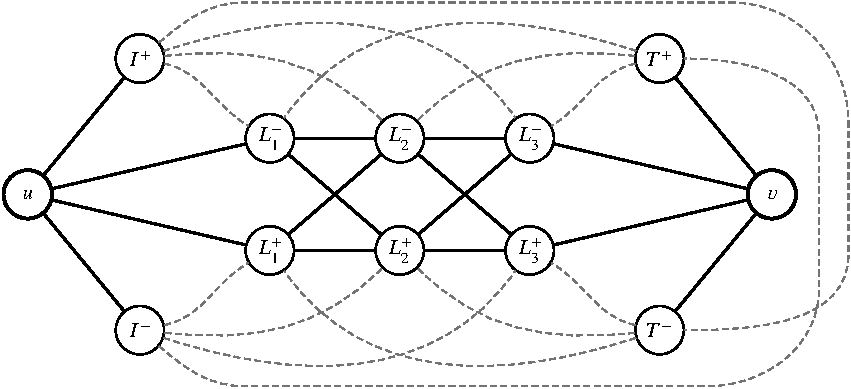
\includegraphics{transition-graph.pdf}
    \caption{The transition graph by type of chain link: solid edges can remain in $G \setminus P$, dashed edges never do}
    \label{fig:transition-graph}
\end{figure}

\paragraph{No $u$--$v$ path.}
Suppose that $G \setminus P$ contains a $u$--$v$ path $Q$.
The internal vertices of a connecting path have degree two, so $Q$ contains a connecting path either as a whole or not at all.
By the first paragraph, each end of a connecting path contained in $Q$ is $u$, $v$, or a vertex of an unused path, and between two consecutive connecting paths $Q$ stays on a single unused path.
The edges of $G \setminus P$ at $u$ and at $v$ belong to connecting paths.
Hence the connecting paths of $Q$, in their order along $Q$, form a walk from $u$ to $v$ in $\Gamma$ whose vertices other than $u$ and $v$ are unused paths.
Let $W$ be a $u$--$v$ path of $\Gamma$ contained in this walk.

Since $P$ is consistent, the unused paths of all chain links of a block have the same sign.
Every edge of type~(b) or~(c) joins two paths of opposite signs in one block, so one of its ends is not an unused path, and $W$ contains no such edge (dashed in Figure~\ref{fig:transition-graph}).
The edges of types~(a) and~(d) join a vertex $I_i^{\sigma}$ only to $u$ and a vertex $T_i^{\sigma}$ only to $v$, and none of them joins $u$ to $v$.
Hence $W$ has internal vertices, all of them are paths of literal chain links, and all edges of $W$ are of type~(d).
A path of $L_{j,k}$ lies on edges of type~(d) only for the clause $C_k$, so $W$ is the path $u, L_{1,k}^{s(\ell_1)}, L_{2,k}^{s(\ell_2)}, L_{3,k}^{s(\ell_3)}, v$ of some clause $C_k = (\ell_1 \vee \ell_2 \vee \ell_3)$ and passes through three literal chain links.
All three paths $L_{j,k}^{s(\ell_j)}$ are then unused, so $P$ does not hit the clause thread of $C_k$.
This contradicts Lemma~\ref{lem:clause-threads}, because $\tau$ satisfies every clause.

Therefore $G \setminus P$ contains no $u$--$v$ path, and $P$ is separating.
\end{proof}

\begin{theorem}
\label{thm:ssp-np-complete}
The \SSP{} problem is NP-complete.
\end{theorem}

\begin{proof}
The reduction is Algorithm~\ref{alg:reduction}.
We show that it is correct and runs in polynomial time, and that \SSP{} belongs to NP.

\paragraph{Correctness.}
The constructed instance of \SSP{} is equivalent to the original \ThreeSAT{} instance:
\begin{enumerate}[(a)]
    \item If there exists a separating shortest path $P$ in $G$, then a satisfying assignment for the original \ThreeSAT{} instance can be extracted from $P$.

    Since $P$ is a shortest $u$--$v$ path, it is a chain path by Lemma~\ref{lem:chain-paths}, and since it is separating, it hits every thread.
    By Lemma~\ref{lem:synchronization}, $P$ is consistent, so it determines a truth assignment $\tau$.
    Since $P$ also hits every clause thread, $\tau$ satisfies at least one literal in every clause by Lemma~\ref{lem:clause-threads}.
    Thus, $\tau$ is a satisfying assignment for the original formula.

    \item If there exists a satisfying assignment for the \ThreeSAT{} instance, then a separating shortest path in $G$ can be constructed from it.

    Given a satisfying assignment $\tau$, let $P$ be the consistent chain path of $\tau$.
    The path $P$ is a shortest $u$--$v$ path (Lemma~\ref{lem:chain-paths}), and it hits every thread (Lemmas~\ref{lem:synchronization} and~\ref{lem:clause-threads}).
    By Lemma~\ref{lem:separating}, $P$ is separating, so $G\setminus P$ contains no $u$--$v$ path.
\end{enumerate}

\paragraph{Running time of the reduction.}
The reduction runs in polynomial time.
The chain has $2n+3m$ chain links, and the construction creates $2n+7m$ threads, each of which has at most three crossing edges and at most four connecting paths.
Before the calibration, the chain therefore has $O(n+m)$ edges.
Balancing the two paths of a chain link adds at most two edges for each of its crossing edges, so $\Lambda = O(n+m)$.
Finally, each of the $O(n+m)$ connecting paths is subdivided until it has $\Lambda$ edges, which adds $O((n+m)^2)$ edges in total.
Hence, the size of $G$ and the running time of Algorithm~\ref{alg:reduction} are polynomial in the input size.

\paragraph{Membership in NP.}
A candidate path $P$ is verified in polynomial time by checking that $P$ is a shortest $u$--$v$ path, removing its edges from $G$, and testing by breadth-first search whether a $u$--$v$ path remains.
Hence \SSP{} belongs to NP.
\end{proof}

In the graph $G$ constructed by Algorithm~\ref{alg:reduction}, every vertex other than $u$ and $v$ has degree at most three.
The ends of the chain links and of the crossing edges have degree three, and all remaining vertices other than $u$ and $v$ have degree two.
On the other hand, $c(u,v) \geq 2n + 7m$, because the threads are edge-disjoint $u$--$v$ paths, and $d(u,v) = \Lambda$.
Hence the reduction gives no hardness result for instances with bounded $c(u,v)$ or bounded $d(u,v)$.

\subsection{From Separating Shortest Path to Min Cut-Path}\label{sec:ssp-to-mcp}
The second step reduces \SSP{} to \MinCutPath, which we state in decision form.

\begin{problem}[\MinCutPath{} (Decision Version)]
Let $G=(V,E)$ be an undirected graph and $u,v \in V$ distinct vertices.
Cut-paths are defined in Definition~\ref{def:cut-path}.
The decision version of the \MinCutPath{} problem is defined as follows:

\begin{center}
\begin{tabular}{p{0.12\linewidth}p{0.8\linewidth}}
\textbf{Input:} & A graph $G=(V,E)$, vertices $u,v \in V$, and an integer $b$. \\
\textbf{Question:} & Does there exist a cut-path $S \subseteq E$ between $u$ and $v$ with $|S|\leq b$?
\end{tabular}
\end{center}
\end{problem}

\begin{theorem}
\label{thm:mcp-np-complete}
The decision version of the \MinCutPath{} problem is NP-complete.
\end{theorem}

\begin{proof}
We reduce \SSP{} to the decision version of \MinCutPath{} and use Theorem~\ref{thm:ssp-np-complete}.

\paragraph{Reduction.}
Let $G$ be an instance of \SSP{} with distinguished vertices $u,v$.
We set the threshold $b := d(u,v)$, which is defined because $u$ and $v$ lie in the same connected component (Section~\ref{sec:fundamentals}), and ask whether $G$ admits a cut-path of size at most $b$.
The threshold $b$ is computed by breadth-first search, so the reduction runs in polynomial time.

\paragraph{Correctness.}
Suppose that $G$ admits a separating shortest path $P$.
Then $|P| = d(u,v) = b$, and $P$ itself is a cut-path of size $b$, since (i) it is a $u$--$v$ path and (ii) its removal disconnects $u$ from $v$, so $P$ is also a $u$--$v$ cut.
Conversely, suppose that $G$ has a cut-path $S$ with $|S| \leq b$.
Then $S$ contains a $u$--$v$ path $P$, which has at least $d(u,v) = b$ edges, so $S = P$, and $P$ is a shortest $u$--$v$ path in $G$.
Since $S$ also contains a $u$--$v$ cut, $G \setminus P$ contains no $u$--$v$ path.
Hence $P$ is a separating shortest path, and the two instances are equivalent.

\paragraph{Membership in NP.}
A candidate cut-path $S$ can be verified in polynomial time by checking that $|S| \leq b$, that $S$ contains a $u$--$v$ path, and that $G\setminus S$ contains no $u$--$v$ path (e.g., by breadth-first search).

\paragraph{Conclusion.}
\MinCutPath{} is in NP, and the NP-complete problem \SSP{} (Theorem~\ref{thm:ssp-np-complete}) reduces to it in polynomial time.
\end{proof}

The decision version is NP-complete, and hence the optimization version is NP-hard.

\begin{corollary}
\label{cor:lower-bound-attained}
It is NP-complete to decide, for a graph $G$ and two distinct vertices $u, v$ of $G$, whether $\cp(u, v) = d(u, v)$.
\end{corollary}

\begin{proof}
By Lemma~\ref{lem:basic-bounds}, $\cp(u, v) \geq d(u, v)$, and by the proof of Theorem~\ref{thm:mcp-np-complete}, equality holds if and only if $G$ contains a separating shortest $u$--$v$ path.
Hence the question is the \SSP{} problem, which is NP-complete by Theorem~\ref{thm:ssp-np-complete}.
\end{proof}

\section{Approximation Hardness}
\label{sec:approximation}

By Corollary~\ref{cor:two-approximation}, the union of a minimum $u$--$v$ cut and a shortest $u$--$v$ path is a cut-path with at most $2\cp(u,v) - 1$ edges, so a minimum cut-path is approximated within a factor of two in polynomial time.

A \emph{polynomial-time approximation scheme} (PTAS) for \MinCutPath{} is an algorithm that, given a graph $G = (V, E)$, two distinct vertices $u, v \in V$ and a number $\epsilon > 0$, returns a cut-path between $u$ and $v$ with at most $(1+\epsilon)\cp(u,v)$ edges, in time polynomial in $|V|$ for every fixed $\epsilon$.
It is a \emph{fully polynomial-time approximation scheme} (FPTAS) if its running time is polynomial in $|V|$ and $1/\epsilon$.

The reduction of Section~\ref{sec:np-completeness} excludes a PTAS.
Let $G$, $u$ and $v$ be the output of Algorithm~\ref{alg:reduction} for a formula with $n$ variables and $m$ clauses.
For a $u$--$v$ path $P$ of $G$, let $\eta(P)$ denote the number of threads that share no edge with $P$, and let $\eta^{*}$ be the minimum of $\eta(P)$ over all chain paths $P$.

\begin{lemma}
\label{lem:missed-threads}
Every cut-path between $u$ and $v$ in $G$ has at least $\Lambda + \eta^{*}$ edges.
\end{lemma}

\begin{proof}
Let $S$ be a cut-path between $u$ and $v$, and let $P \subseteq S$ be a $u$--$v$ path.
The set $S \setminus P$ is a $u$--$v$ cut of $G \setminus P$ (Section~\ref{sec:fundamentals}), and every thread that shares no edge with $P$ is a $u$--$v$ path of $G \setminus P$.
Any two threads are edge-disjoint, so $S \setminus P$ contains a separate edge of each of these threads, and $|S| \geq |P| + \eta(P)$.
We show that $|P| + \eta(P) \geq \Lambda + \eta^{*}$.

If $P$ is a chain path, then $|P| = \Lambda$ and $\eta(P) \geq \eta^{*}$.
Otherwise, as in the proof of Lemma~\ref{lem:chain-paths}, $P$ contains every connecting path either as a whole or not at all.
It contains $k \geq 1$ connecting paths, each with $\Lambda$ edges, and all its other edges are edges of the chain.
The two paths of a chain link form a cycle, so $P$ contains at most one of them.
Let $\widetilde{P}$ be the chain path that traverses, in every chain link, the path of the link that is contained in $P$ if there is one, and the positive path otherwise.
Let $x$ be the number of crossing edges of $P$ that do not lie on $\widetilde{P}$, and let $h$ be the number of single edges of the chain that lie on $P$.
Then $|P| \geq k\Lambda + x + h$.
A thread consists of its connecting paths and its crossing edges.
Hence a thread that shares an edge with $P$ but no edge with $\widetilde{P}$ contains one of the $k$ connecting paths of $P$ or one of these $x$ crossing edges.
Every connecting path and every crossing edge belongs to exactly one thread, so there are at most $k + x$ such threads, and $\eta(P) \geq \eta(\widetilde{P}) - k - x \geq \eta^{*} - k - x$.
Together,
\[
|P| + \eta(P) \geq k\Lambda + h + \eta^{*} - k = \Lambda + \eta^{*} + (k-1)(\Lambda - 1) + h - 1.
\]
A chain with a chain link has at least two single edges, so $\Lambda \geq 2$.
If $k \geq 2$, the right-hand side is therefore at least $\Lambda + \eta^{*}$.
If $k = 1$, the connecting path of $P$ does not join $u$ and $v$ (proof of Lemma~\ref{lem:chain-paths}), so $P$ has an edge of the chain at $u$ or at $v$.
The only edges of the chain at $u$ and at $v$ are single edges, so $h \geq 1$, and the right-hand side is again at least $\Lambda + \eta^{*}$.
\end{proof}

\begin{lemma}
\label{lem:unsatisfied-clauses}
Suppose that every variable has at most five occurrences in the formula.
Let $P$ be a chain path, and let $\tau$ be the truth assignment with $\tau(x_i) = \mathsf{true}$ if and only if $P$ traverses the positive path of $I_i$.
Then $\tau$ satisfies all but at most $5\,\eta(P)$ clauses.
\end{lemma}

\begin{proof}
To every clause that $\tau$ does not satisfy we assign a thread that $P$ does not hit, so that at most five clauses receive the same thread.
Let $C_k = (\ell_1 \vee \ell_2 \vee \ell_3)$ be a clause that $\tau$ does not satisfy.
If $P$ does not hit the clause thread of $C_k$, we assign this thread to $C_k$.
Otherwise $P$ traverses, for some $j$, the path of $L_{j,k}$ with the sign $s(\ell_j)$.
Let $x_i$ be the variable of $\ell_j$.
Since $\tau$ does not satisfy $\ell_j$, the path $P$ traverses in $I_i$ the path with the sign opposite to $s(\ell_j)$, so it traverses paths of opposite signs in $I_i$ and in $L_{j,k}$.
If $P$ traverses paths of opposite signs in $I_i$ and in $T_i$, it does not hit one of the two 2-synchronization threads of $x_i$, by the first item in the proof of Lemma~\ref{lem:synchronization}.
Otherwise it does not hit one of the two 3-synchronization threads of $L_{j,k}$, by the second item.
We assign such a thread to $C_k$.
A clause thread and a 3-synchronization thread of $L_{j,k}$ are assigned only to the clause $C_k$, and a 2-synchronization thread of $x_i$ only to clauses in which $x_i$ occurs, of which there are at most five.
\end{proof}

\begin{theorem}
\label{thm:no-ptas}
There is a constant $\epsilon_0 > 0$ such that, unless $\mathrm{P} = \mathrm{NP}$, no polynomial-time algorithm returns, for every graph $G = (V, E)$ and every two distinct vertices $u, v \in V$, a cut-path between $u$ and $v$ with fewer than $(1+\epsilon_0)\cp(u,v)$ edges.
In particular, \MinCutPath{} has no PTAS unless $\mathrm{P} = \mathrm{NP}$.
\end{theorem}

\begin{proof}
Consider formulas in which every clause contains three literals with distinct variables and every variable occurs in exactly five clauses.
Feige~\cite[Proposition~2.1.2]{Feige1998Threshold} showed that, for some constant $\delta > 0$, it is NP-hard to distinguish the satisfiable formulas of this kind from those in which every truth assignment leaves at least $\delta m$ clauses unsatisfied.
Let $\epsilon_0 = \delta/200$, and let $G$, $u$ and $v$ be the output of Algorithm~\ref{alg:reduction} for such a formula.

Every variable has five occurrences, so $5n = 3m$.
A path of a chain link has two edges before the threadings, and every threading through it adds two edges.
By Algorithm~\ref{alg:reduction}, six threads are threaded through each of the two paths of $I_i$ and of $T_i$, and one and two threads through the two paths of a literal chain link.
After the calibration, the paths of $I_i$ and $T_i$ therefore have $14$ edges, and those of a literal chain link have six.
With the $2n + 3m + 1$ single edges of the chain,
\[
\Lambda = (2n + 3m + 1) + 14 \cdot 2n + 6 \cdot 3m = 39m + 1 \leq 40m.
\]

If the formula is satisfiable, then $G$ contains a separating shortest $u$--$v$ path (Lemma~\ref{lem:separating}), which is a cut-path with $d(u,v) = \Lambda$ edges, and $\cp(u,v) = \Lambda$ by Lemma~\ref{lem:basic-bounds}.
If every truth assignment leaves at least $\delta m$ clauses unsatisfied, then $\eta^{*} \geq \delta m / 5$ by Lemma~\ref{lem:unsatisfied-clauses}, and by Lemma~\ref{lem:missed-threads},
\[
\cp(u,v) \geq \Lambda + \frac{\delta m}{5} \geq \Bigl(1 + \frac{\delta}{200}\Bigr)\Lambda = (1+\epsilon_0)\Lambda.
\]
An algorithm as in the statement returns a cut-path with fewer than $(1+\epsilon_0)\Lambda$ edges in the first case and with at least $(1+\epsilon_0)\Lambda$ edges in the second.
The graph $G$ is constructed in polynomial time (Theorem~\ref{thm:ssp-np-complete}), and $\Lambda = d(u,v)$ is computed by breadth-first search.
Hence the algorithm distinguishes the two cases in polynomial time, and $\mathrm{P} = \mathrm{NP}$.
A PTAS with $\epsilon = \epsilon_0/2$ is such an algorithm.
\end{proof}

\begin{corollary}
\label{cor:no-fptas}
Unless $\mathrm{P} = \mathrm{NP}$, there is no FPTAS for \MinCutPath.
\end{corollary}

\begin{proof}
For every fixed $\epsilon$, the running time of an FPTAS is polynomial in $|V|$.
Hence every FPTAS is a PTAS, and the claim follows from Theorem~\ref{thm:no-ptas}.
\end{proof}

We do not know whether a polynomial-time algorithm achieves a constant factor smaller than two.

\section{Graphs of Diameter Two}
\label{sec:diameter-two}

The first class in which the problem can be solved in polynomial time consists of the graphs of diameter two.

\begin{definition}[Diameter]
\label{def:diameter}
A graph $G = (V, E)$ has \emph{diameter at most $k$} if $d(x, y) \leq k$ for every pair of vertices $x, y \in V$.
The smallest such $k$ is the \emph{diameter} of $G$, denoted by $\diam(G)$.
\end{definition}

We derive a formula for $\cp(u,v)$ in graphs of diameter two, which yields a polynomial-time algorithm (Remark~\ref{rem:algorithm}).
The proof uses a decomposition.
In any graph, a cut $C$ induces a partition of the vertex set into four subsets $I, J, K, L$.
Each vertex lies on one of the two sides $A_1, A_2$ of the cut, and it is either incident to an edge of the cut or not.

\begin{definition}[Decomposition Induced by a Cut]
\label{def:cut-decomposition}
Let $G = (V, E)$ be a graph, and let $C$ be a cut that divides $G$ into two sets $A_1$ and $A_2$ (i.e., $V = A_1 \cup A_2$, $A_1 \cap A_2 = \emptyset$, and $C$ is the set of all edges between $A_1$ and $A_2$).
The \emph{decomposition induced by $C$} consists of the four sets $I, J, K, L$ such that:
\begin{itemize}
    \item $I \cup J = A_1$ and $I \cap J = \emptyset$,
    \item $K \cup L = A_2$ and $K \cap L = \emptyset$,
    \item every vertex of $J \cup K$ is incident to an edge of $C$,
    \item no vertex of $I \cup L$ is incident to an edge of $C$.
\end{itemize}
\end{definition}

In a graph of diameter two, the vertices that are not incident to the cut lie on at most one side of it.

\begin{lemma}
\label{lem:empty-i-or-l}
Let $G = (V, E)$ be a graph of diameter at most two, let $C$ be a cut that divides $G$ into two sets $A_1$ and $A_2$, and let $I, J, K, L$ be the decomposition induced by $C$ (Definition~\ref{def:cut-decomposition}).
Then at least one of the sets $I$ and $L$ is empty:
\[
I = \emptyset \quad\text{or}\quad L = \emptyset.
\]
\end{lemma}

\begin{proof}
Suppose, for a contradiction, that there are vertices $x \in I$ and $y \in L$.
Since $x \in A_1$, $y \in A_2$ and $C$ is the set of all edges between $A_1$ and $A_2$, every $x$--$y$ path contains an edge $\{a, b\}$ of $C$ with $a \in A_1$ and $b \in A_2$.
The vertices $a$ and $b$ are incident to an edge of $C$, so $a \in J$ and $b \in K$.
In particular, $a \neq x$ and $b \neq y$, because $x$ and $y$ are not incident to any edge of $C$.
Hence the path has at least one edge between $x$ and $a$, the edge $\{a, b\}$, and at least one edge between $b$ and $y$, so it passes through $J$ and $K$ and has at least three edges.
Therefore $d(x, y) \geq 3$, which contradicts the assumption that $G$ has diameter at most two.
\end{proof}

\begin{lemma}
\label{lem:odd-intersection}
Let $G = (V, E)$ be a graph, and let $u, v \in V$ be two distinct vertices.
Let $C$ be the set of all edges between two sets $A_1$ and $A_2$ that partition $V$, with $u \in A_1$ and $v \in A_2$, and let $P$ be a path that connects $u$ and $v$.
Then the path $P$ contains an odd number of edges of $C$:
\[
|C \cap P| \equiv 1 \pmod{2}.
\]
\end{lemma}

\begin{proof}
When we traverse the path $P$ from $u$ to $v$, each edge of $C \cap P$ changes the side of the cut (i.e., it switches between $A_1$ and $A_2$), while every other edge of $P$ stays on the same side.
The path starts in $A_1$ and ends in $A_2$.
If the path crossed the cut an even number of times, its first and its last vertex would lie on the same side, which contradicts the assumption that $u \in A_1$ and $v \in A_2$.
Therefore, the path crosses the cut an odd number of times, so $|C \cap P|$ is odd.
\end{proof}

\begin{theorem}
\label{thm:diameter-two}
Let $G = (V, E)$ be a graph of diameter at most two, and let $u, v \in V$ be two distinct vertices.
Then a minimum cut-path between $u$ and $v$ has
\[
\cp(u, v) = c(u, v) + d(u, v) - 1
\]
edges.
\end{theorem}

\begin{proof}
We distinguish two cases based on the values of $d(u, v)$ and $c(u, v)$.
Since $G$ has diameter at most two, it is connected, so $c(u, v) \geq 1$ and $d(u, v) \in \{1, 2\}$.
Hence the two cases below cover all pairs $u, v$.

\emph{Case 1: $d(u, v) = 1$ or $c(u, v) = 1$.}
By Lemma~\ref{lem:basic-bounds}, in this case we have
\[
\cp(u, v) = c(u, v) + d(u, v) - 1.
\]

\emph{Case 2: $d(u, v) = 2$ and $c(u, v) \geq 2$.}
By Lemma~\ref{lem:basic-bounds},
\[
c(u, v) \leq \cp(u, v) \leq c(u, v) + 2 - 1 = c(u, v) + 1.
\]
Suppose, for a contradiction, that $\cp(u, v) = c(u, v)$, which by the bounds above is the only alternative to $\cp(u, v) = c(u, v) + 1$.
Then a minimum cut-path $S$ has the same size as a minimum cut.
The set $S$ contains a $u$--$v$ cut, which has at least $c(u, v) = |S|$ edges, so this cut is all of $S$.
Hence the set $S$ itself is a minimum cut, which we denote by $C$, and the $u$--$v$ path $P$ contained in $S$ is a subset of this cut.

The cut $C$ is the set of all edges between a vertex set and its complement, with $u$ and $v$ on different sides.
Indeed, let $A$ be the vertex set of the component of $G \setminus C$ that contains $u$.
Every edge between $A$ and $V \setminus A$ belongs to $C$, since otherwise its end outside $A$ would lie in the same component as $u$.
These edges separate $u$ from $v$, because $v \notin A$.
By the minimality of $C$, there are at least $|C|$ of them, so they form all of $C$.
We denote the two sides $A$ and $V \setminus A$ by $A_1$ and $A_2$, in either order.

By Lemma~\ref{lem:odd-intersection}, applied to $C$ and to the path $P \subseteq C$, the number of edges of $P$ is odd.
Since $d(u,v) = 2$, the path $P$ has at least two edges, and hence at least three.

Let $I, J, K, L$ be the decomposition induced by the cut $C$ (Definition~\ref{def:cut-decomposition}).
By Lemma~\ref{lem:empty-i-or-l}, after exchanging the names $A_1$ and $A_2$ (and with them $I$ with $L$ and $J$ with $K$) if necessary, we may assume that $L = \emptyset$.
The cut $C$, the path $P$ and the relation $P \subseteq C$ are symmetric in $u$ and $v$.
Hence we may also assume, after exchanging the names of $u$ and $v$ if necessary, that $u \in A_2$.
Since $A_2 = K \cup L = K$, we have $u \in K$, so $V$ is partitioned into the three sets $I, J, K$.
Here $v \in J$, because the last edge of $P$ belongs to the cut and is incident to $v$, so the vertex $v$ cannot belong to the set $I$.
Figure~\ref{fig:diameter-two-structure} shows this structure.

\begin{figure}[H]
    \centering
    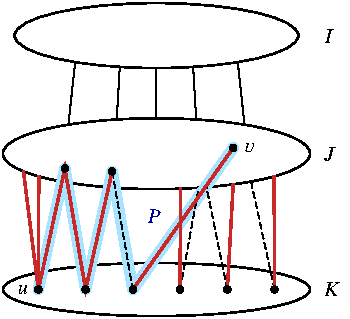
\includegraphics{diameter-two-structure.pdf}
    \caption{The cut $C$ in the proof of Theorem~\ref{thm:diameter-two}: the path $P$ is shaded, the counted edges are red}
    \label{fig:diameter-two-structure}
\end{figure}

Every edge of $C$ has exactly one end in $K$, because $C$ is the set of all edges between $A_1 = I \cup J$ and $A_2 = K$.
For a vertex $x$ and a vertex set $W$, let $\deg(x, W)$ denote the number of neighbors of $x$ in $W$.
The vertex $u$ has no neighbors in $I$, because an edge between $u \in A_2$ and a vertex of $I \subseteq A_1$ would belong to $C$, but no vertex of $I$ is incident to an edge of $C$.
We count the edges of $C$ according to their end-vertex in $K$, in three groups:
\begin{enumerate}[(i)]
    \item The vertex $u$ is incident to $\deg(u, J)$ edges of $C$, the edges that lead from $u$ to the opposite side of the cut.

    \item The path $P$ is contained in the cut and has at least three edges, so its vertices alternate between $A_2$ and $A_1$.
    Hence its third vertex lies in $K$ and differs from $u$, because a path does not repeat vertices.
    This vertex contributes at least two edges to the cut, namely the second and the third edge of $P$.

    \item Each of the remaining $|K| - 2$ vertices of the set $K$ is incident to an edge of $C$ by the definition of $K$, so it contributes at least one edge to the cut.
\end{enumerate}
Since $u \in K$ is not its own neighbor, we have $\deg(u, K) \leq |K| - 1$.
Since $V = I \cup J \cup K$ and $u$ has no neighbors in $I$, we have $\deg(u) = \deg(u, J) + \deg(u, K)$.
Hence
\begin{align*}
\cp(u, v) = c(u, v) = |C| &\geq \underbrace{\deg(u, J)}_{\text{(i)}} + \underbrace{2}_{\text{(ii)}} + \underbrace{|K| - 2}_{\text{(iii)}}\\
&\geq \deg(u, J) + \deg(u, K) + 1 = \deg(u) + 1 \geq c(u, v) + 1.
\end{align*}
The last inequality holds because the edges incident to $u$ form a $u$--$v$ cut.
This contradicts the assumption that $\cp(u, v) = c(u, v)$.
Hence $\cp(u, v) = c(u, v) + 1 = c(u, v) + d(u, v) - 1$.
\end{proof}

\begin{remark}
\label{rem:algorithm}
Whenever $\cp(u, v) = c(u, v) + d(u, v) - 1$, the proof of Lemma~\ref{lem:basic-bounds} shows that the union of an arbitrary minimum $u$--$v$ cut and an arbitrary shortest $u$--$v$ path is a minimum cut-path.
Hence, in graphs of diameter two, a minimum cut-path can be found by one minimum-cut computation and one breadth-first search.
\end{remark}

\begin{corollary}
\label{cor:diameter-two-degrees}
Let $G = (V, E)$ be a graph of diameter at most two, and let $u, v \in V$ be two distinct vertices.
Then $c(u, v) = \min\{\deg(u), \deg(v)\}$, and hence $\cp(u, v) = \min\{\deg(u), \deg(v)\} + d(u, v) - 1$.
\end{corollary}

\begin{proof}
The edges incident to $u$ form a $u$--$v$ cut, and so do the edges incident to $v$, so $c(u, v) \leq \min\{\deg(u), \deg(v)\}$.
Let $C$ be a minimum $u$--$v$ cut.
As in the proof of Theorem~\ref{thm:diameter-two}, $C$ is the set of all edges between two sides $A_1$ and $A_2$ that partition $V$, and by Lemma~\ref{lem:empty-i-or-l} we may name the sides so that every vertex of $A_2$ is incident to an edge of $C$.
Let $w$ be the one of the vertices $u, v$ that lies in $A_2$, and let $\deg(w, W)$ again denote the number of neighbors of $w$ in a vertex set $W$.
Every edge of $C$ has exactly one end in $A_2$.
The vertex $w$ is an end of $\deg(w, A_1)$ of them, and each of the other $|A_2| - 1$ vertices of $A_2$ is an end of at least one.
Hence $|C| \geq \deg(w, A_1) + |A_2| - 1 \geq \deg(w, A_1) + \deg(w, A_2) = \deg(w)$, so $c(u, v) \geq \min\{\deg(u), \deg(v)\}$.
The formula for $\cp(u, v)$ follows from Theorem~\ref{thm:diameter-two}.
\end{proof}

Hence the edges incident to the one of the vertices $u, v$ with the smaller degree form a minimum $u$--$v$ cut, and a minimum cut-path is found in linear time, without a minimum-cut computation.

\section{Cactus Graphs}
\label{sec:cut-two}

The same formula holds in connected graphs in which the cut-value of every pair of vertices is at most two.

These are the \emph{cactus graphs}, the connected graphs in which any two distinct cycles share at most one vertex (Lemma~\ref{lem:cactus}).
Such a graph consists of cycles and single edges, any two of which share at most one vertex, an articulation point.

\begin{lemma}
\label{lem:cactus}
A graph $G = (V, E)$ satisfies $c(x, y) \leq 2$ for every pair of distinct vertices $x, y \in V$ if and only if any two distinct cycles of $G$ share at most one vertex.
\end{lemma}

\begin{proof}
Let $c(x, y) \leq 2$ for every pair of distinct vertices, and suppose first that two distinct cycles share an edge.
Then the second cycle contains a path whose ends $x \neq y$ lie on the first cycle and whose edges do not belong to the first cycle.
To find it, take an edge of the second cycle that is not on the first, and follow the second cycle from it in both directions up to the first vertex of the first cycle.
The two vertices reached are distinct, because the second cycle contains both ends of the shared edge.
The union of the two cycles then contains the two vertices $x$ and $y$ joined by three edge-disjoint paths, namely this path and the two $x$--$y$ paths along the first cycle.
Separating $x$ from $y$ then requires at least three edges, which contradicts the assumption $c(x,y) \leq 2$.
Similarly, two edge-disjoint cycles cannot share two vertices $x \neq y$, because they would contain four edge-disjoint $x$--$y$ paths.

Conversely, suppose that any two distinct cycles of $G$ share at most one vertex.
Two vertices in different components have cut-value zero, so let $x, y$ be two distinct vertices joined by a path $P$, and let $e_1$ be the edge of $P$ at $x$.
If $e_1$ lies on no cycle, then it is a bridge, and its removal separates $x$ from $y$.
Otherwise let $Z$ be a cycle through $e_1$, and let $e_2$ be the other edge of $Z$ at $x$.
Suppose that $G \setminus \{e_1, e_2\}$ contains an $x$--$y$ path $Q$.
Following $P$ from $x$ to its first vertex other than $x$ that lies on $Q$, and returning to $x$ along $Q$, we obtain a cycle that contains $e_1$ and not $e_2$.
This cycle and $Z$ are distinct and share both ends of $e_1$, a contradiction.
Hence $c(x, y) \leq 2$.
\end{proof}

\begin{theorem}
\label{thm:cut-two}
Let $G = (V, E)$ be a cactus graph.
Then, for any two distinct vertices $u,v \in V$, a minimum cut-path between $u$ and $v$ has
\[
\cp(u, v) = c(u, v) + d(u, v) - 1
\]
edges.
\end{theorem}

\begin{proof}
We distinguish two cases based on the values of $d(u, v)$ and $c(u, v)$.
Since $G$ is connected, $c(u, v) \geq 1$, and $c(u, v) \leq 2$ by Lemma~\ref{lem:cactus}.
Since $u \neq v$, we have $d(u, v) \geq 1$.
Hence the two cases below cover all pairs $u, v$.

\emph{Case 1: $d(u, v) = 1$ or $c(u, v) = 1$.}
The formula holds by Lemma~\ref{lem:basic-bounds}.

\emph{Case 2: $d(u, v) \geq 2$ and $c(u, v) = 2$.}
By Lemma~\ref{lem:basic-bounds}, we have
\[
d(u, v) \leq \cp(u, v) \leq d(u, v) + 1.
\]
Suppose, for a contradiction, that $\cp(u, v) = d(u, v)$.
A minimum cut-path $S$ then has $d(u, v)$ edges and contains a $u$--$v$ path, which has at least $d(u, v)$ edges, so $S$ is this path.
Hence a minimum cut-path is a shortest $u$--$v$ path $P$ that contains a $u$--$v$ cut, so the graph $G \setminus P$ contains no $u$--$v$ path.

Since $c(u, v) = 2$, no single edge separates $u$ from $v$.
A bridge of $G$ on the path $P$ would separate $u$ from $v$, so no edge of $P$ is a bridge, and every edge of $P$ lies on a cycle of the cactus graph $G$.
By Lemma~\ref{lem:cactus}, this cycle is unique, since two cycles through the same edge would share two vertices.

Let $Z_1, Z_2, \dots, Z_t$ be the cycles that contain the edges of $P$, in the order in which $P$ traverses them, a cycle being listed again if $P$ comes back to it.
In each cycle $Z_i$, the path $P$ follows one of the two arcs between the vertex where it enters $Z_i$ and the vertex where it leaves $Z_i$.
The path $P$ does not return to a cycle $Z_i$ after leaving it.
Otherwise the part of $P$ from the vertex where it leaves $Z_i$ to the next vertex of $Z_i$ on $P$, together with an arc of $Z_i$, would be a second cycle that shares an edge with $Z_i$, which contradicts Lemma~\ref{lem:cactus}.
Hence the cycles $Z_1, \dots, Z_t$ are pairwise distinct, and the edges of $P$ on $Z_i$ are exactly the edges of this arc.

The path $P$ enters $Z_1$ at $u$ and leaves $Z_t$ at $v$.
For $i < t$, the vertex where $P$ leaves $Z_i$ is the vertex where it enters $Z_{i+1}$, since every edge of $P$ lies on one of these cycles.
The other arc of each cycle $Z_i$ is edge-disjoint from $P$, and consecutive arcs share these vertices, so these arcs form a $u$--$v$ walk in $G \setminus P$, which contains a $u$--$v$ path.
This contradicts the assumption that $P$ contains a $u$--$v$ cut.
Therefore,
\[
\cp(u, v) = d(u, v) + 1 = c(u, v) + d(u, v) - 1. \qedhere
\]
\end{proof}

By Remark~\ref{rem:algorithm}, a minimum cut-path in such a graph is again obtained as the union of a minimum cut and a shortest path.

\begin{example}
\label{ex:strict}
In both graphs of Figure~\ref{fig:counterexamples}, the three red edges form a $u$--$v$ path whose removal separates $u$ from $v$, so $\cp(u, v) = 3$.
In the left graph, $c(u, v) = 2$ and $d(u, v) = 3$, and in the right graph, $c(u, v) = 3$ and $d(u, v) = 2$.
In both, $c(u, v) + d(u, v) - 1 = 4$, so the upper bound of Lemma~\ref{lem:basic-bounds} is not attained.
Hence the hypothesis of Theorem~\ref{thm:cut-two} cannot be weakened to $c(u, v) \leq 2$, and that of Theorem~\ref{thm:diameter-two} cannot be weakened to $d(u, v) \leq 2$.
\end{example}

\begin{figure}[H]
    \centering
    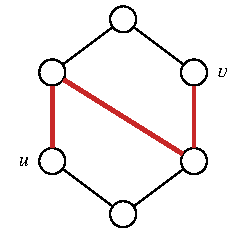
\includegraphics{counterexample-cut-two.pdf}\qquad\qquad
    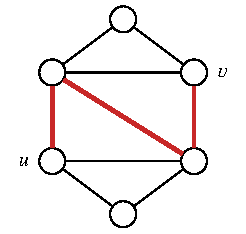
\includegraphics{counterexample-distance-two.pdf}
    \caption{Two graphs with $\cp(u,v) = 3 < c(u,v) + d(u,v) - 1$; the cut-path is red}
    \label{fig:counterexamples}
\end{figure}

\section{Erdős–Rényi Graphs}
\label{sec:random-graphs}

We study the \MinCutPath{} problem in Erdős–Rényi random graphs $G(n, p)$, in which each of the possible edges on $n$ vertices is present independently with probability $p$.
Throughout this section, $\log$ denotes the natural logarithm.
An event holds \emph{with high probability} if its probability tends to one as $n \to \infty$.

Random graphs with a constant edge probability $p$, called dense, have diameter two with high probability.
This fact is well known~\cite[Exercise~1.4.8]{Frieze2016}, and we include its short proof.

\begin{theorem}
\label{thm:random-diameter-two}
Let $0 < p < 1$ be a constant.
Then
\[
\lim_{n \to \infty} \mathbb{P}\bigl(\diam(G(n, p)) = 2\bigr) = 1.
\]
\end{theorem}

\begin{proof}
Let $x$ and $y$ be two distinct vertices.
Each of the other $n - 2$ vertices is adjacent to both $x$ and $y$ with probability $p^2$, independently of the others, so $x$ and $y$ have no common neighbor with probability $(1 - p^2)^{n-2}$.
By the union bound over the fewer than $n^2$ pairs of vertices, the probability that some two vertices have no common neighbor is at most $n^2 (1 - p^2)^{n-2}$, which tends to zero.
Hence $\diam(G(n, p)) \leq 2$ with high probability.
The graph $G(n, p)$ is complete, that is, has diameter one, with probability $p^{n(n-1)/2}$, which also tends to zero.
\end{proof}

By Theorem~\ref{thm:diameter-two} and Remark~\ref{rem:algorithm}, a minimum cut-path in a graph of diameter two has $c(u, v) + d(u, v) - 1$ edges and can be computed in polynomial time.
Consequently, for dense random graphs, the \MinCutPath{} problem can be solved exactly in polynomial time with high probability.

Consider now sparse Erdős–Rényi random graphs $G(n, p)$ with $p = \alpha \log n / n$, where $\alpha > 1$ is a constant.
We write $G$ for $G(n,p)$.
For such graphs, we use two known results, on the diameter~\cite{ChungLu2001} and on the edge connectivity~\cite{Bollobas2001}.

\begin{theorem}[Diameter~\cite{ChungLu2001}]
\label{thm:random-diameter}
Let $p = \alpha \log n / n$ with a constant $\alpha > 1$.
Then
\[
\lim_{n\to\infty} \mathbb{P}\left( \diam(G) \leq \frac{\log n}{\log \log n} \right) = 1.
\]
\end{theorem}

Chung and Lu~\cite{ChungLu2001} proved that, with high probability, $\diam(G) \leq \lceil \log((33\alpha^2/400)\, n \log n) / \log(\alpha \log n) \rceil + 2$ for $\alpha > 1$.
The right-hand side is at most $\log n / \log \log n$ for all sufficiently large $n$.
Chung and Lu define the diameter of a disconnected graph as that of its largest component.
For $\alpha > 1$, the graph $G$ is connected with high probability (Lemma~\ref{lem:connectivity-bounds}), so the bound holds for $\diam(G)$ in the sense of Definition~\ref{def:diameter}.

\begin{theorem}[{Connectivity~\cite[p.~169]{Bollobas2001}}]
\label{thm:random-connectivity}
Let $p = \alpha \log n / n$ with a constant $\alpha > 1$.
Then, with high probability, the edge connectivity of $G$ equals its minimum degree $\delta(G)$.
\end{theorem}

\begin{lemma}[Degree Bounds]
\label{lem:degree-bounds}
Let $p = \alpha \log n / n$ with a constant $\alpha > 1$.
Then there exists a constant $\beta_1 > 0$, depending only on $\alpha$, such that
\[
\lim_{n\to\infty} \mathbb{P}\Bigl( \forall x \in V(G): \ \deg(x) \geq \beta_1 \log n \Bigr) = 1.
\]
\end{lemma}

\begin{proof}
The degree of a fixed vertex $x$ has the binomial distribution with mean $\mu = (n-1)p = (1-o(1))\,\alpha \log n$.
For $a > 0$, let $h(a) = a \log a - a + 1$.
By the Chernoff bound (see, e.g.,~\cite[Eq.~(21.19)]{Frieze2016}),
\[
\mathbb{P}\bigl(\deg(x) \leq a\mu\bigr) \leq \exp(-\mu h(a)) \quad \text{for } 0 < a < 1.
\]
Since $h(a) \to 1$ as $a \to 0$ and $\alpha > 1$, we can fix a constant $0 < a_1 < 1$ such that $\alpha h(a_1) > 1$.
For this constant, the probability above is $o(1/n)$, because $\exp(-\mu h(a_1)) = n^{-(1-o(1))\,\alpha h(a_1)}$.

The union bound over all $n$ vertices shows that, with high probability, every degree is at least $a_1 \mu$.
Since $\mu = (1 - 1/n)\,\alpha \log n \geq \alpha \log n / 2$ for $n \geq 2$, the claim follows, for instance, with $\beta_1 = a_1 \alpha / 2$.
\end{proof}

\begin{lemma}
\label{lem:connectivity-bounds}
Let $p = \alpha \log n / n$ with a constant $\alpha > 1$, and let $\beta_1$ be the constant from Lemma~\ref{lem:degree-bounds}.
Then
\[
\lim_{n\to\infty} \mathbb{P}\Bigl( \forall u \neq v: \ c(u,v) \geq \beta_1 \log n \Bigr) = 1.
\]
\end{lemma}

\begin{proof}
By Theorem~\ref{thm:random-connectivity} and Lemma~\ref{lem:degree-bounds}, with high probability, the edge connectivity of $G$ equals its minimum degree $\delta(G)$ and all its degrees are at least $\beta_1 \log n$.
Suppose that both events hold.
Then every cut separating two distinct vertices has at least $\delta(G)$ edges, so all pairs of distinct vertices $u, v$ satisfy
\[
c(u, v) \geq \min_{x \neq y} c(x, y) \geq \min_{z \in V(G)} \deg(z) \geq \beta_1 \log n. \qedhere
\]
\end{proof}

\begin{theorem}
\label{thm:approximation-scheme}
Let $p \geq \alpha \log n / n$ with a constant $\alpha > 1$, and let $\beta_1$ be the constant from Lemma~\ref{lem:degree-bounds}.
Then, with high probability, every two distinct vertices $u, v$ of $G(n, p)$, every minimum $u$--$v$ cut $C$ and every shortest $u$--$v$ path $P$ satisfy
\[
|C \cup P| \leq \Bigl(1 + \frac{1}{\beta_1 \log \log n}\Bigr)\, \cp(u, v).
\]
In particular, for every $\epsilon > 0$, the algorithm that returns the union of a minimum $u$--$v$ cut and a shortest $u$--$v$ path is an average $(1+\epsilon)$-approximation scheme for the \MinCutPath{} problem on the inputs $(G(n, p), u, v)$, for an arbitrary choice of the two distinct vertices $u, v$.
\end{theorem}

\begin{proof}
Adding edges to a graph cannot increase the distances and cannot decrease the values $c(u,v)$.
The bounds of Theorem~\ref{thm:random-diameter} and Lemma~\ref{lem:connectivity-bounds} are stated for $p = \alpha \log n / n$.
Hence, by the standard coupling of the random graphs $G(n,p)$ for different edge probabilities (see, e.g.,~\cite[Section~1.1]{Frieze2016}), they remain valid for every $p \geq \alpha \log n / n$.
Thus, with high probability, all pairs of distinct vertices $u,v$ satisfy
\[
d(u,v) \leq \diam(G) \leq \frac{\log n}{\log \log n}
\qquad\text{and}\qquad
c(u,v) \geq \beta_1 \log n.
\]
Suppose that this event holds, let $u, v$ be two distinct vertices, and let $S = C \cup P$ for a minimum $u$--$v$ cut $C$ and a shortest $u$--$v$ path $P$.
By the proof of Lemma~\ref{lem:basic-bounds}, the set $S$ is a cut-path with $|S| \leq c(u,v) + d(u,v) - 1$.
By Lemma~\ref{lem:basic-bounds}, the minimum cut is no larger than the minimum cut-path, that is, $c(u,v) \leq \cp(u,v)$.
Hence
\begin{align*}
\frac{|S|}{\cp(u,v)} &\leq \frac{c(u,v)+d(u,v)-1}{c(u,v)} \leq \frac{c(u,v)+d(u,v)}{c(u,v)} = 1 + \frac{d(u,v)}{c(u,v)}\\
&\leq 1+\frac{\log n / \log \log n}{\beta_1 \log n} = 1 + \frac{1}{\beta_1 \log \log n},
\end{align*}
which proves the first claim.

For the second claim, the algorithm runs in polynomial time, since both a minimum cut and a shortest path can be computed in polynomial time~\cite{Cormen2022}.
For an input $X = (G, u, v)$, its output is the set $S$ above, and $\OPT(X) = \cp(u,v)$.
The bound $1 + 1/(\beta_1 \log \log n)$ is smaller than $1+\epsilon$ for all sufficiently large $n$.
Thus, the algorithm achieves the approximation ratio $1+\epsilon$ on a set of inputs whose probability tends to one, so it is an average $(1+\epsilon)$-approximation scheme.
\end{proof}

\section{Fixed-Parameter Tractability}
\label{sec:fpt}

A decision problem is \emph{fixed-parameter tractable} (FPT) with respect to a parameter $b$ of its instances if it can be decided in time $f(b)$ times a polynomial in the size of the instance, for some computable function $f$ (see, e.g.,~\cite{Marx2013Separators}).
The \emph{parameterized version} of \MinCutPath{} is its decision version (Section~\ref{sec:ssp-to-mcp}) with the threshold $b$ as the parameter.
It asks, for a graph $G = (V, E)$, two distinct vertices $u, v \in V$ and an integer $b$, whether there is a cut-path between $u$ and $v$ with at most $b$ edges.

By Lemma~\ref{lem:basic-bounds}, an instance with $d(u,v) > b$ or $c(u,v) > b$ is a no-instance, and an instance with $c(u,v) + d(u,v) - 1 \leq b$ is a yes-instance.
Both values are computed in polynomial time~\cite{Cormen2022}.

For a $u$--$v$ cut $C$, let $d_C(u,v)$ denote the minimum of $|P \setminus C|$ over all $u$--$v$ paths $P$.
It is the distance between the images of $u$ and $v$ in the graph obtained from $G$ by contracting the edges of $C$.

\begin{lemma}
\label{lem:contraction}
Let $G = (V, E)$ be a graph, and let $u, v \in V$ be two distinct vertices. Then
\[
\cp(u,v) = \min_{C}\, \bigl(|C| + d_C(u,v)\bigr),
\]
where the minimum is over all inclusion-minimal $u$--$v$ cuts $C$.
\end{lemma}

\begin{proof}
For every $u$--$v$ cut $C$ and every $u$--$v$ path $P$, the set $C \cup P$ is a cut-path with $|C| + |P \setminus C|$ edges, so $\cp(u,v) \leq |C| + d_C(u,v)$.
Conversely, a minimum cut-path $S$ contains a $u$--$v$ path $P$ and a $u$--$v$ cut, hence also an inclusion-minimal $u$--$v$ cut $C$, and
\[
|C| + d_C(u,v) \leq |C| + |P \setminus C| = |C \cup P| \leq |S| = \cp(u,v). \qedhere
\]
\end{proof}

By Lemma~\ref{lem:contraction}, one can decide whether $\cp(u,v) \leq b$ by computing $d_C(u,v)$ for every inclusion-minimal $u$--$v$ cut $C$ with at most $b$ edges, each time by a shortest-path computation in which the edges of $C$ have length zero.
This algorithm runs in time $|E|^{O(b)}$ and is not an FPT algorithm, because a graph that consists of $b$ internally disjoint $u$--$v$ paths with $|E|/b$ edges each has $(|E|/b)^b$ inclusion-minimal $u$--$v$ cuts with $b$ edges.
We avoid the enumeration.
After the remaining parts of the graph are replaced by weighted shortcuts, all these cuts lie in a graph of treewidth bounded by a function of $b$.

We use tree decompositions, treewidth and the monadic second-order logic of graphs as in~\cite[Section~2.1]{Marx2013Separators}, and write $\tw(H)$ for the treewidth of a graph $H$.
For a set $N$ of vertices of $H$, the graph $H - N$ is obtained from $H$ by deleting the vertices of $N$.
Let $x, y$ be two distinct vertices of $H$.
A set $N \subseteq V(H) \setminus \{x, y\}$ \emph{separates} $x$ from $y$ in $H$ if $x$ and $y$ lie in different components of $H - N$.
Such a set is an \emph{$x$--$y$ separator}, and it is \emph{minimal} if none of its proper subsets is an $x$--$y$ separator.
For $D \subseteq V(H)$, the graph $\torso(H, D)$ has the vertex set $D$, and two vertices $a, a' \in D$ are adjacent in it if they are adjacent in $H$ or if $H$ contains an $a$--$a'$ path whose internal vertices lie outside $D$~\cite[Definition~2.5]{Marx2013Separators}.

\begin{lemma}[{\cite[Proposition~2.7, Lemma~2.11 and Remark~2.13]{Marx2013Separators}}]
\label{lem:treewidth-reduction}
There are functions $f_1$ and $g_1$ and an algorithm with the following property.
Given a graph $H$, two distinct non-adjacent vertices $x, y$ of the same component of $H$, and an integer $k$ such that $H$ has an $x$--$y$ separator with at most $k$ vertices, the algorithm computes in time $f_1(k) \cdot (|V(H)| + |E(H)|)$ a set $D \subseteq V(H)$ with $x, y \in D$ such that
\begin{enumerate}[(a)]
    \item $D$ contains every minimal $x$--$y$ separator of $H$ with at most $k$ vertices,
    \item $\tw(\torso(H, D)) \leq g_1(k)$, and
    \item a set $N \subseteq D \setminus \{x, y\}$ separates $x$ from $y$ in $\torso(H, D)$ if and only if it separates $x$ from $y$ in $H$.
\end{enumerate}
\end{lemma}

Marx, O'Sullivan and Razgon~\cite[Lemma~2.11]{Marx2013Separators} construct the set $D \setminus \{x, y\}$ and bound the bramble number of its torso, which is the treewidth plus one.
Their bounds on the running time and on the bramble number depend on the minimum size of an $x$--$y$ separator, which is at most $k$, and on the difference between $k$ and this size, so they are bounded by functions of $k$.
By their Remark~2.13, adding $x$ and $y$ increases the treewidth by at most two.
Statement~(c) is their Proposition~2.7.

\paragraph{Construction.}
Let $(G, u, v, b)$ be an instance with $c(u,v) \leq b$.
Let $G'$ be the graph obtained from $G$ by subdividing every edge $e \in E$ with a new vertex $z_e$, and let $R_F = \{z_e : e \in F\}$ for $F \subseteq E$.
Deleting the vertex $z_e$ from $G'$ corresponds to removing the edge $e$ from $G$.
Hence a set $F \subseteq E$ is a $u$--$v$ cut of $G$ if and only if $R_F$ separates $u$ from $v$ in $G'$, and $R_F$ is a minimal $u$--$v$ separator of $G'$ whenever $F$ is an inclusion-minimal $u$--$v$ cut of $G$.
The vertices $u$ and $v$ are not adjacent in $G'$ and lie in the same component, and $G'$ has a $u$--$v$ separator with $c(u,v) \leq b$ vertices.
We apply Lemma~\ref{lem:treewidth-reduction} to $G'$ with $x = u$, $y = v$ and $k = b$ and obtain a set $D$.
By~(a), $z_e \in D$ for every edge $e$ of an inclusion-minimal $u$--$v$ cut of $G$ with at most $b$ edges.

Let $G_D = \torso(G', D)$.
For an edge $aa'$ of $G_D$, let $\omega(aa')$ be the minimum number of vertices of $R_E$ among the internal vertices of an $a$--$a'$ path of $G'$ whose internal vertices lie outside $D$.
In particular, $\omega(aa') = 0$ if $a$ and $a'$ are adjacent in $G'$.
Let $G_D^+$ be the graph obtained from $G_D$ by replacing every edge $aa'$ with $\omega(aa') \geq 1$ by an $a$--$a'$ path with $\min\{\omega(aa'), b+1\}$ new internal vertices.
Let $Y$ be the set of all new vertices, and let $B = R_E \cap D$.
Subdividing edges does not change which vertices of $D$ lie in a common component after vertices of $D$ are deleted.
Together with~(c) and the correspondence between the cuts of $G$ and the separators of $G'$, this gives, for every $F \subseteq E$ with $R_F \subseteq D$,
\begin{equation}
\label{eq:cut-separator}
\text{$F$ is a $u$--$v$ cut of $G$ if and only if $R_F$ separates $u$ from $v$ in $G_D^+$.}
\end{equation}
A set $M \subseteq B \cup Y$ is \emph{good} if
\begin{enumerate}[(i)]
    \item $M \cap B$ separates $u$ from $v$ in $G_D^+$, and
    \item $G_D^+$ contains a $u$--$v$ path all of whose vertices in $B \cup Y$ belong to $M$.
\end{enumerate}

\begin{lemma}
\label{lem:good-set}
Let $(G, u, v, b)$ be an instance with $c(u,v) \leq b$, and let $G_D^+$, $B$ and $Y$ be constructed as above.
Then $\cp(u,v) \leq b$ if and only if there is a good set with at most $b$ vertices.
\end{lemma}

\begin{proof}
Suppose first that $\cp(u,v) \leq b$.
By Lemma~\ref{lem:contraction}, there are an inclusion-minimal $u$--$v$ cut $C$ and a $u$--$v$ path $P$ of $G$ with $|C| + |P \setminus C| \leq b$.
Since $|C| \leq b$, we have $R_C \subseteq D$ and hence $R_C \subseteq B$.
Let $P'$ be the $u$--$v$ path of $G'$ obtained from $P$ by subdividing its edges, and let $u = a_0, a_1, \dots, a_r = v$ be the vertices of $P'$ that lie in $D$, in their order on $P'$.
For $1 \leq i \leq r$, the part of $P'$ between $a_{i-1}$ and $a_i$ has no internal vertex in $D$.
Hence $a_{i-1}a_i$ is an edge of $G_D$, and $\omega(a_{i-1}a_i)$ is at most the number of internal vertices of this part that lie in $R_E$.
Every such vertex is $z_e$ for an edge $e \in P$ with $z_e \notin D$, and then $e \notin C$.
In particular, $\omega(a_{i-1}a_i) \leq |P \setminus C| \leq b$, so $G_D^+$ contains a $u$--$v$ path $Q$ that passes through $a_0, \dots, a_r$ in this order and has exactly $\omega(a_{i-1}a_i)$ vertices of $Y$ between $a_{i-1}$ and $a_i$.
Let $M = R_C \cup \bigl(V(Q) \cap (B \cup Y)\bigr)$.
Condition~(ii) holds by the choice of $M$.
Condition~(i) holds because $M \cap B \supseteq R_C$ and $R_C$ separates $u$ from $v$ in $G_D^+$ by~\eqref{eq:cut-separator}.
The vertices of $Q$ in $B$ are the vertices $z_e \in D$ with $e \in P$, the number of vertices of $Q$ in $Y$ is at most the number of edges $e \in P$ with $z_e \notin D$, and $z_e \in D$ for every $e \in C$.
Hence
\[
|M| \leq |C| + |\{e \in P \setminus C : z_e \in D\}| + |\{e \in P \setminus C : z_e \notin D\}| = |C| + |P \setminus C| \leq b.
\]

Conversely, let $M$ be a good set with $|M| \leq b$, and let $Q$ be a $u$--$v$ path of $G_D^+$ as in~(ii).
Let $F_1 = \{e \in E : z_e \in M \cap B\}$.
By~(i) and~\eqref{eq:cut-separator}, $F_1$ is a $u$--$v$ cut of $G$.
The path $Q$ consists of edges $aa'$ of $G_D$ with $\omega(aa') = 0$ and of paths that replace edges $aa'$ of $G_D$ with $\omega(aa') \geq 1$.
The internal vertices of such a path lie in $Y$, hence in $M$ by~(ii).
Since $|M| \leq b$, their number is not $b+1$, so it is $\omega(aa')$.
In both cases we replace the part of $Q$ between $a$ and $a'$ by an $a$--$a'$ path of $G'$ whose internal vertices lie outside $D$ and exactly $\omega(aa')$ of them in $R_E$.
The result is a $u$--$v$ walk $Q'$ in $G'$.
Let $F_2 = \{e \in E : z_e \in V(Q')\}$.
A vertex $z_e$ of $Q'$ is a vertex of $Q$ in $B$, and then $e \in F_1$ by~(ii), or it is an internal vertex of one of the inserted paths, and the number of these vertices is at most $|V(Q) \cap Y| \leq |M \cap Y|$.
Hence $|F_1 \cup F_2| \leq |M \cap B| + |M \cap Y| = |M| \leq b$.
In $G'$, the vertex $z_e$ is adjacent exactly to the two ends of $e$, so any two vertices of $V$ that follow each other on $Q'$ are equal or are the two ends of an edge of $F_2$, and $F_2$ contains a $u$--$v$ path.
Thus $F_1 \cup F_2$ is a cut-path between $u$ and $v$ with at most $b$ edges.
\end{proof}

\begin{theorem}
\label{thm:fpt}
\MinCutPath{} is fixed-parameter tractable with respect to the threshold $b$.
\end{theorem}

\begin{proof}
The algorithm computes $c(u,v)$ and rejects if $c(u,v) > b$, which is correct by Lemma~\ref{lem:basic-bounds}.
Otherwise it constructs $G'$, $D$, $G_D$, $\omega$ and $G_D^+$ and accepts if and only if there is a good set with at most $b$ vertices, which is correct by Lemma~\ref{lem:good-set}.

The graph $G'$ has $|V| + |E|$ vertices and $2|E|$ edges, so $D$ is computed in time $f_1(b) \cdot (|V| + 3|E|)$.
For two vertices $a, a' \in D$, a shortest-path computation in $G' - (D \setminus \{a, a'\})$, in which the length of a path is the number of its internal vertices in $R_E$, decides whether $aa'$ is an edge of $G_D$ and gives $\omega(aa')$.
Hence $G_D^+$ is constructed in polynomial time and has at most $|D| + (b+1)|D|^2$ vertices.

Subdividing an edge $aa'$ of a graph $H$ by a vertex $w$ yields a graph of treewidth at most $\max\{\tw(H), 2\}$.
Indeed, a tree decomposition of $H$ has a bag that contains $a$ and $a'$, and a new bag $\{a, a', w\}$ attached to it gives a tree decomposition of the new graph.
Hence $\tw(G_D^+) \leq \max\{\tw(G_D), 2\} \leq \max\{g_1(b), 2\}$ by~(b).

Let $W$ be a set of vertices of $G_D^+$ with $v \in W$.
The vertex $v$ is reachable from $u$ by a path whose vertices other than $u$ lie in $W$ if and only if every set of vertices that contains $u$ and every vertex of $W$ adjacent to one of its members also contains $v$.
This condition is a formula of monadic second-order logic.
Condition~(ii) is this condition for $W = M \cup \bigl(V(G_D^+) \setminus (B \cup Y)\bigr)$, condition~(i) is its negation for $W = V(G_D^+) \setminus (M \cap B)$, and $|M| \leq b$ holds if and only if there are $b$ vertices, not necessarily distinct, such that every member of $M$ is one of them.
Hence the existence of a good set with at most $b$ vertices is expressed by a formula $\varphi_b$ of monadic second-order logic over graphs with the vertex labels $u$, $v$, $B$ and $Y$.
By Courcelle's theorem~\cite[Theorem~2.2]{Marx2013Separators} and its extension to graphs with vertex labels stated there, a property expressed by such a formula $\varphi$ is decided on a graph $H$ in time $f_\varphi(\tw(H)) \cdot (|V(H)| + |E(H)|)$.
The total running time is therefore $f(b)$ times a polynomial in $|V| + |E|$, for a function $f$ of $b$.
\end{proof}

The proof gives no explicit bound on $f$.
We do not know whether \MinCutPath{} can be solved in time $2^{O(b)}$ times a polynomial in $|V| + |E|$.

\section{Conclusion}
\label{sec:conclusion}

The union of a minimum $u$--$v$ cut and a shortest $u$--$v$ path is a minimum cut-path in graphs of diameter two and in cactus graphs.
In random graphs with edge probability at least $\alpha \log n / n$, for a constant $\alpha > 1$, it is within a factor $1 + o(1)$ of the minimum with high probability, and in every graph it is within a factor of two (Corollary~\ref{cor:two-approximation}).
In general graphs, deciding whether $\cp(u, v) = d(u, v)$ is NP-complete (Corollary~\ref{cor:lower-bound-attained}), and some constant factor larger than one cannot be achieved in polynomial time unless $\mathrm{P} = \mathrm{NP}$ (Theorem~\ref{thm:no-ptas}).
The decision version is fixed-parameter tractable with respect to the threshold $b$, with no explicit bound on the dependence of the running time on $b$ (Theorem~\ref{thm:fpt}).

We leave the following questions open.
\begin{enumerate}
    \item What is the complexity of deciding whether $\cp(u, v) = c(u, v)$?

    \item What is the complexity of \MinCutPath{} for bounded $c(u, v)$ or bounded $d(u, v)$?
    Both values grow with the formula in the graphs of our reduction (Section~\ref{sec:ssp}).

    \item Is \MinCutPath{} NP-hard on graphs of diameter three?
    Finding a matching cut and, for unit edge lengths, finding the most vital edges for shortest paths are solvable in polynomial time on graphs of diameter two and NP-hard on graphs of diameter three~\cite{Bazgan2019MostVital,LeLe2019MatchingCut}.

    \item Can \MinCutPath{} be solved in polynomial time on the graphs in which every pair of vertices is at distance at most two or has cut-value at most two?
    This class contains the graphs of diameter two and the cactus graphs, but the formula $\cp(u, v) = c(u, v) + d(u, v) - 1$ does not hold in it (Example~\ref{ex:strict}).

    \item Can \MinCutPath{} be solved in polynomial time on planar graphs?
    In a planar graph, every minimal edge cut corresponds to a cycle in the dual graph and vice versa, and several problems on cuts and flows can be solved faster in planar graphs than in general ones~\cite{itai1979maximum,henzinger1997faster}.

    \item Can a minimum cut-path be approximated in polynomial time within a constant factor smaller than two?

    \item Can the decision version be solved in time $2^{O(b)}$ times a polynomial in the size of the graph?
\end{enumerate}


\section*{Acknowledgments}

The author thanks Martin Loebl, who proposed the \MinCutPath{} problem, for his guidance and for valuable discussions.

\bibliographystyle{cas-model2-names}

\bibliography{references}

\end{document}
